\documentclass{article}
\author{S.T. Countryman, Y.S. Asali, E. Calamari, A. Lam, M.C. McGrae-Menge}
\usepackage[utf8]{inputenc}
\usepackage[colorlinks, urlcolor=cyan]{hyperref}
% display code; from: https://stackoverflow.com/questions/3175105/writing-code-in-latex-document
\usepackage{listings}
\usepackage{color}
\usepackage{geometry}
\usepackage{graphicx}
\usepackage{wrapfig}

\definecolor{dkgreen}{rgb}{0,0.6,0}
\definecolor{gray}{rgb}{0.5,0.5,0.5}
\definecolor{mauve}{rgb}{0.58,0,0.82}

\lstset{frame=tb,
  aboveskip=3mm,
  belowskip=3mm,
  showstringspaces=false,
  columns=flexible,
  basicstyle={\small\ttfamily},
  numbers=none,
  numberstyle=\tiny\color{gray},
  keywordstyle=\color{blue},
  commentstyle=\color{dkgreen},
  stringstyle=\color{mauve},
  breaklines=true,
  breakatwhitespace=true,
  tabsize=3
}

\title{LHO January 2019 Site Visit Report}

\definecolor{todo}{RGB}{170, 86, 73}        % light rust
\newcommand*{\TODO}{\textcolor{todo}}

\begin{document}
\maketitle

\begin{abstract}
    Members of Columbia University's LSC group (GECo) visited the LIGO Hanford Observatory (LHO) between January 3 and January 18, 2019, to ensure that LHO's Timing System was ready for aLIGO's third observing run (O3). Timing System tasks are described and the work done summarized in Section~\ref{sec:timing}. In addition to this project, GECo members sought out other on-site tasks (not necessarily timing related) that would help with O3 preparations. The GECo team consisted of undergraduate student researchers Yasmeen Siham Asali, Emily Calamari, Ana Lam, and Madox Carver McGrae-Menge as well as graduate student researcher Stefan Countryman.
\end{abstract}

\section{\label{sec:timing}Timing}

\subsection{\label{sec:cable-lengths}Finish measuring cable lengths/types}

Might need to do 
\href{https://en.wikipedia.org/wiki/Time-domain_reflectometer}{TDR})
to get remaining cable lengths.
\footnote{
    Cable length Google spreadsheet \href{https://docs.google.com/spreadsheets/d/1cjpBtpd4oPAfjNjBhE3RXxSx3ma3oopqLLZFMjEjc0w/edit\#gid=0}{here}, based on \href{https://docs.google.com/spreadsheets/d/1AfZ9m7Qetefmtr-PnHNARC14OWaPfn0z5c9GOvcojyA/edit\#gid=0}{LLO Google spreadsheet} (LLO cable measurements copied \hyperref[sec:llocables]{in the appendix}).
}
You can get the cable names by going to the cable locations and looking for little labels attached to the cables. The cable type will be printed directly onto the cables all along their lengths; RG-58 is a common cable type. You'll need to measure the lengths yourself (don't worry about accuracy better than a foot or so overall). The easily-accessible cables have already been measured, hence the possible need for TDR (see notes after table).
Record cable information in Table~\ref{table:lho-cables}.

We won't be able to take measurements on antenna cables; will need to approximate those with Dave and then maybe TDR them in a more painful measurement later (since we would probably need to disconnect the roof antenae). Alternatively, we could estimate the length to within $\pm10$ feet using the design document for the end station along with an understanding of the routing of the cable from the CNS II to the end station roof antenna (Dave Barker knows how this is routed; he drew 
\hyperref[fig:routing]{a cartoon}, but we'll need to bug him for a more precise routing), though this seems like a lot of trouble for an imprecise measurement. aLOG for 1PPS measurements 
\href{https://alog.ligo-wa.caltech.edu/aLOG/index.php?callRep=43185}{here}. See Fig. \ref{fig:rainertdr} for a pic of Rainer performing a TDR measurement.

\textbf{Update:} We will do this Tuesday, Jan. 15 (maintenance day). We will start at the end stations because, according to Dave, they have their antennae at the edges (while the corner station has its GPS antennae on the weather station, more than 6 feet from the edge, at least at LHO).

\textbf{Update:} Opened \href{https://services.ligo-la.caltech.edu/LHO/workpermits/view.php?permit_id=8044}{work permit 8044} for this work. We will start by measuring the cable lengths at the end stations since this will not require disconnecting anything related to the Timing \textit{Distribution} System.

\textbf{Update:} Filoberto showed Stef how to use a TDR (fig.~\ref{fig:tdr-tool}) to take measurements (Instructions in fig.~\ref{fig:tdr-dtf-instructions}). We tested it in the EE Shop with a 150ft RG-58C/U cable and a GPS antenna (fig.~\ref{fig:tdr-test}) as proof-of-concept; since we can't remove the GPS Antenna at the rooftop end of the cable without getting up to the roof (which requires harness certification), we wanted to check that a DTF (distance to fault) measurement would work with a GPS antenna terminating the cable.

For the distance measurement, we will be using Distance to Fault (DTF) mode, which will require inputting a rough estimate of the distance to the GPS antenna (overestimating is good since this distance specifies the bounds of our distance search; 200ft is probably a good starting point). 

\begin{itemize}
    \item{Get adapters for the GPS antenna cable. The CNS II Clock has a TNC female connector on the back for the antenna (Fig.~\ref{fig:cns-ii-rear}), so we will need a female TNC to female BNC adapter for the TDR measurement.}
    \item{Get the Velocity Factor for whatever cable type is used for the GPS antenna.} The CNS II to VEA antenna patch cable is LMR-195 Like at Livingston with a velocity factor of \href{https://www.pasternack.com/50-ohm-low-loss-flexible-lmr195-pe-jacket-double-shielded-black-lmr-195-p.aspx}{0.8}. The VEA to Roof antenna cable will likely be LMR-400 with a velocity ratio of \href{https://www.febo.com/reference/cable_data.html}{0.85}. 
    \item{Get screwdriver for removing rack-mounted CNS II clock.}
    \item{Grab the TDR tool}
    \item{Uninstall CNS II from rack and leave with Dave Barker}
    \begin{itemize}
        \item At X End
        \item At Y End
    \end{itemize}
    \item{Perform TDR measurement and record cable type and cable name}
    \begin{itemize}
        \item At X End
        \item At Y End
    \end{itemize}
    \item{Perform Further TDR measurement and record cable type and cable name}
    \begin{itemize}
        \item \TODO{X End VEA to Roof GPS Antenna Cable}
        \item \TODO{Y End VEA to Roof GPS Antenna Cable}
    \end{itemize}
    \item{\TODO{In the descriptions below, also mention which ports on the Comparators each RG-58 1PPS cable is connected to.}}
    \item \TODO{Add photos taken at end stations to the appendix.}
\end{itemize}

\textbf{Update 1/15:} We finished measuring the cables that are connected to the CNS II clocks, however, we found that they seem to be patch cables to VEA (based on a bump in TDR found at 90 ft. as well as the cable names). We suspect that the cable in VEA continues up to the rooftop GPS antenna. \TODO{We will need to check the cable type (probably LMR-400) in VEA and measure its length}. We can also measure the 1PPS cable length for the CNS II clock while we are in VEA. We wrote \href{https://alog.ligo-wa.caltech.edu/aLOG/index.php?callRep=46442}{aLOG 46442} describing our activity (Appendix~\ref{sec:cns-ii-removal-alog}).

\textbf{Update 1/17:} We went to EX VEA to find the GPS antenna cable from VEA to roof. We couldn't find it, but we do have the absolute timing delay between roof and CNS II clock of ~270', calculated from a TDR measurement of ~215' with a velocity factor of 0.8 for LMR-195 (see above). We wrote \href{https://alog.ligo-wa.caltech.edu/aLOG/index.php?callRep=46499}{an aLOG} describing our activity.

\begin{center}
  \label{table:lho-cables}
  \begin{tabular}{ | l | l | l | l | }
    \hline
    \textbf{Description}  			            & \textbf{Length [ft]} 	& \textbf{Type} & \textbf{Cable Name} \\ \hline
    Cs-III 1PPS to Comparator Port 1            & 5 					& RG-58			& C50-005-0019 \\ \hline
    S350 NTP Server 1PPS to Comparator Port 2   & 5 					& RG-58			& C50-005-0025 \\ \hline
    58503B GPS Clock 1PPS to Comparator Port 3  & 5 					& RG-58			& SYMMETRICOM\_1PPS \\ \hline
    Trimble to Master 1PPS cable	            & 2 					& RG-58			& \\ \hline
    Timing Master GPS Antenna Cable	            &  						& 				& \\ \hline
    Trimble GPS Antenna Cable                   &  						& 				& \\ \hline
    Lightning arrestor to Trimble               &  						& 				& \\ \hline
    Lightning arrestor to Master                &  						& 				& \\ \hline
    Y-End CNS II 1PPS  				            & 29 					& RG-58 		& CDS\_GPS\_COMPARATOR \\ \hline
    Y-End CNS II GPS to VEA                     & 90					& LMR-195		& CDS\_GPS\_ANT\_VEA \\ \hline
    Y-End VEA to Rooftop GPS Antenna            &                       &               & \\ \hline
    X-End CNS II 1PPS				            & 29					& RG-58			& CDS\_GPS\_COMPARATOR \\ \hline
    X-End CNS II GPS to VEA                     & 90					& LMR-195		& CDS\_GPS\_ANT\_VEA \\ \hline
    X-End VEA to Rooftop GPS Antenna            &                       &               & \\
    \hline
  \end{tabular}
\end{center}

The S350 Network Time Server datasheet can be found \href{https://www.microsemi.com/document-portal/doc_view/133759-syncserver-s350-network-time-server-datasheet}{here}. The Symmetricom 58503B GPS clock (in MSR) datasheet can be found \href{https://accusrc.com/uploads/datasheets/4975_58503b.pdf}{here}.

\TODO{\subsection{Remove CNS II Clocks for Firmware Upgrade}}

Ask Dave if the end station Timing \textit{Diagnostic} System CNS II Clocks should be updated to fix the midnight firmware bug issue. There has been some confusion about whether this needs fixing, but during our last visit, Dave Barker said it is probably not worth updating the CNS II firmware given that we haven't seen any other problems besides the midnight bugs. Since then, Dave emailed about it so we should check one more time whether or not it is important. Rick Hambly said it would take 2 weeks to update. 

\textbf{Update:} After much back-and-forth (Appendix~\ref{sec:midnightbug}), we've decided to remove the CNS II Clocks and return them to the manufacturer for firmware updates. We removed these as part of the cable-length measurement task (Sec.~\ref{sec:cable-lengths}) and left them with Dave Barker for shipping. The X-End CNS-II has serial number 404358 (Fig.~\ref{fig:cns-ii-ex-bottom}). The Y-End CNS-II has serial number 404357 (Fig.~\ref{fig:cns-ii-ey-bottom}).

\TODO{Give Dave Barker the shipping information for the CNS-II return for firmware reprogramming.}

\TODO{
\subsection{\label{sec:update-timing-diagram}
    Update or confirm
    \href{https://dcc.ligo.org/LIGO-D1500201}{installed timing map at LHO} (GitHub repo
    \href{https://github.com/stefco/geco_channels}{here}).
}
}
\textbf{Note:} The items below are from the last visit and still need to be done, but you'll need to check the installation \textit{again} to confirm that things have not changed since the last visit in August 2018. You can edit the files with Omnigraffle 6, which can be downloaded straight from \href{https://downloads.omnigroup.com/software/MacOSX/10.10/OmniGraffle-6.6.2.dmg}{this link}.

\begin{itemize}
  \item{Remove TCT/TCG from LHO diagrams}
  \item{Add cable lengths to both diagrams}
  \item{\TODO{Add cable types to both diagrams via legend}}
  \item{\TODO{Add links to 1PPS diagnostic channels}}
  \item{\TODO{Add some photos to LHO and LLO maps}}
  \item{\TODO{Upload saved changes to DCC}}
\end{itemize}

\subsection{Calibrate atomic clock}

Download a few months of atomic clock (i.e. Cesium clock) data in order to see if it's drifting significantly. If the clock is drifting quickly away from the actual GPS time, then the Cesium clock must be recalibrated. You can download the Cesium clock data using the \href{https://github.com/stefco/geco_data/blob/master/geco_gwpy_dump.py}{\texttt{geco\_gwpy\_dump.py}} script from the \href{https://github.com/stefco/geco_data}{\texttt{geco\_data} git repository}. Use
\hyperref[sec:jobspec]{this jobspec file from the appendix} (copy the contents to \texttt{jobspec.json} and use it with \texttt{geco\_gwpy\_dump.py} as detailed in that scripts help instructions).
Use \hyperref[sec:plottingcode]{this plotting code from the appendix} to visualize the drift rate.

\textit{Last time we came to Hanford, we were unable to calibrate the atomic clock because the signal was being processed through a faulty independent commercial timing system we used for our diagnostic system. The failed module, an old \textit{Time Code Generator} (TCG), was producing truly horrible results for the last few months before the visit (as seen in Fig. \ref{fig:cesium}), making it impossible to calibrate the atomic clock (since the Cs-III signal is fed through the TCG). Dave Barker \href{https://alog.ligo-wa.caltech.edu/aLOG/index.php?callRep=43200}{routed the 1PPS directly from the Cs-III to the comparator} on August 2, 2018, so we should have enough data to calibrate in January 2019.}

\textbf{Update:} We measured a drift coefficient of -11e-15 (Fig.~\ref{fig:cesium}). \textbf{We do not recommend recalibrating the clock at this time}. The current drift behavior is gradual and piecewise-linear (as expected) and will in no way interfere with the short-timescale phase noise measurements that the Cs-III is used for. The current calibration is sufficiently good that the shorter timescale (likely environmentally-caused) piecewise-linear drift of the Cs-III clock is larger than the long-term drift, meaning that further calibration will likely amount to over-fitting and will not produce a qualitative improvement in long-term drift. 

\subsection{Check that the Timing System firmware versions are up-to-date using 
\href{https://wiki.ligo.org/RemoteAccess/RemoteEPICS}{MEDM screens}}

FPGA Firmware versions are on \href{https://awiki.ligo-wa.caltech.edu/wiki/TimingFpgaCode}{Daniel Sigg's aLIGO wiki}. Instructions for this check are on the \href{https://github.com/stefco/geco_docs/blob/master/3-timing-fpga-code.md}{Geco Docs github} page.

\textbf{Update 1/15:} The firmware versions of all the elements of the timing system are up to date. Version information is listed in appendix \ref{sec:firmware}.

\subsection{\label{subsec:medmviewers} Make sure Local- and Remote-MEDM Viewers Match}

Check local MEDM viewers (i.e. the MEDM viewers installed on the workstations on site) and make sure the timing screens etc. match what we see with \href{https://wiki.ligo.org/RemoteAccess/RemoteEPICS}{RemoteMEDM} (you should check this on your own laptop).

\textit{When we went in August 2018, the MEDM Summary screens at the bottom of the page were out of date. Specifically, the end station ones were wrong in their 1PPS descriptions and the corner stations \textbf{might} have been wrong; would have to check that against the installation in MSR. The Remote and Local MEDM screens otherwise matched.}

\subsection{Check which MEDM screen MSR 1PPS descriptions were correct}

See Sec.~\ref{subsec:medmviewers} for information on checking the MEDM screens. We went in to MSR at 1:30pm local on 1/16 (\href{https://alog.ligo-wa.caltech.edu/aLOG/index.php?callRep=46477}{aLOG here}) and checked on the physical connections between diagnostic timing devices and the Timing Comparator module. We recorded which input ports are connected to which diagnostic devices in the table in Sec.~\ref{sec:cable-lengths}.

\textbf{Update 1/17:} Fixed the MEDM summary screens. See my email to Dave (Appendix~\ref{sec:medm-email}) and \href{https://alog.ligo-wa.caltech.edu/aLOG/index.php?callRep=46500}{an aLOG} I wrote.

\textbf{Update 1/17:} The 1PPS labels on the timing overview page has been updated, Dave Barker helped Yasmeen commit the changes that Stefan wrote. 

\subsection{\label{sec:fix-local-medm-readonly}Fix the \texttt{READONLY}-mode MEDM Screen for the Timing Master}

Currently, in \texttt{READONLY} mode at the site, the list of devices connected to the Master does not show up (Fig.~\ref{fig:medm-readonly}; it's possible to pick between "READONLY" and "MASTER" at the top level sitemap, Fig.~\ref{fig:medm-expert-vs-readonly}). It \textit{does} show up when using the \texttt{EXPERT} mode (Fig.~\ref{fig:medm-expert}). When accessing the screens using remote MEDM viewer, either of those buttons work. The \texttt{READONLY} screen is otherwise the same. 

\section{Side Projects}

\TODO{\subsection{DRMI Locking Acquisition System Work}}

After a conversation about the current state of the detector, Sheila Dwyer asked Yasmeen, Ana, Madox, and Emily to look into the DRMI (Dual-Recycling Michelson Interferometer) locking acquisition system. The DRMI is the LIGO instrument without the 4km arms. Many changes to the DRMI locking process have been made recently, yet the success of said alterations had not been objectively delved into. Specifically, within the \texttt{"H1:GRD-ISC\_LOCK\_STATE\_N"} channel we examined both the time durations during the "Lock DRMI 1F" state (denoted by 101) and the success rate of DRMI locks. Trends in the DRMI locking system duration and success rate were cross checked with the aLIGO LHO Logbook. Furthermore, Sheila asked if we could put a summarizing plot on the detchar pages (like \href{https://ldas-jobs.ligo.caltech.edu/~detchar/summary/day/20190111/psl/}{this one}). Generating DetChar summary pages requires creating special \texttt{.ini} configuration files specifying the channels and plot types to be made as well as the location of those plots in the overall summary page structure.

We created scripts for downloading large chunks of data and plotting durations of DRMI locking attempts as requested from Sheila. We generated a plot from August 1 2018 to January 8 2019 which shows the average duration for a locking attempt that were successful and locking attempts that were failures for each hour. With Sheila, we referenced the aLogs for dates that qualitatively appeared to indicate changes in the DRMI locking system's performance within the plot. Sheila would like to have the scripts and instructions on how to use them so that she can use them in the future to assess the DRMI locking system's performance over time spans of a day or time spans of many months.

To Do Items:

\begin{itemize}
    \item \TODO{We will probably need to define a new plot type in the GWpy codebase for this application (since the \texttt{.ini} files must reference an existing GWpy plot type).}
    \item \TODO{We will also need to get Alex Urban or someone to make it possible to have plots with weeks or months of data (vs. the current timespan of a day) since this is the span on which useful conclusions about locking behavior can be gleaned. Sheila already sent an email to Alex on this topic (Appendix~\ref{sec:summary-page-email}).}
    \item Create a Github repository for Sheila with instruction to use the downloading and plotting scripts.
\end{itemize}
\href{https://dcc.ligo.org/LIGO-G1301236}{This slideshow} describes DRMI locking.

\textbf{Update:} We have created a public  \href{https://github.com/ysa2106/LHO_2019}{\texttt{LHO 2019} git repository} with instructions and scripts to run the DRMI locking acquisition analysis. We published an \href{https://alog.ligo-wa.caltech.edu/aLOG/index.php?callRep=46536}{aLOG 46536} detailing our analysis and a significant observation we made that the 30W TCS settings improved locking acquisition.

\TODO{\subsection{Checking for Side-Channel Injections in PCALX Frontend}
}

Keita told us that there are extra injection points in the frontend models for a bunch of channels. These "excitation points" are digital and come before digital filters. The frontends can save data from \textit{before} the excitation point and filter or from \textit{after}; unfortunately, a lot of the data we were recording was only from after the filter, which means we now need to check all of those excitation channels to see whether there were any injections that would have otherwise been undetected. We should also make sure that we only look at observing mode data, i.e. times when the observatory is both ready for observations (\texttt{H1:ODC-MASTER\_CHANNEL\_READY}) and the operator has indicated that we intend to start observing (\texttt{H1:ODC-MASTER\_CHANNEL\_INTENT}). These combine to tell us whether we are in observing mode (\texttt{H1:ODC-MASTER\_CHANNEL\_LATCH}). When in observing mode, any non-zero values in the injection channels we find should be viewed as injections and reported.

A full list of names for excitation channels can be found in Appendix \ref{sec:channels}. Each starts with \texttt{H1:CAL-PCALX\_}, or the Y-end station or LLO equivalent, and the channel names should end in \texttt{EXC}. The timing filters have already been updated so data-viewer no longer shows the excitation point channel names. On MATLAB, these filters are shown in dark green and in dark brown.

To do items:
\begin{itemize}
    \item \TODO{Get old channel names for injection points in timing channels DAC, FPGA, IRIGB}
\end{itemize}

\subsection{Install Jamie's \texttt{ndscope} Project}

Jamie wrote a replacement for DataViewer called \href{https://git.ligo.org/cds/ndscope}{\texttt{ndscope}} that is rapidly supplanting DataViewer at the sites. Because it uses the NDS2 protocol, it can be used off-site, which means that we can install in on our computers and use it to browse channels and get data through a GUI!

\TODO{Screenshots of the models and channels we are interested in for this project will go in the appendix.}

\begin{itemize}
    \item Get \texttt{ndscope} running on MacOS (also required getting \texttt{gpstime})
    \item \TODO{Write a Portfile so that everyone can install it}
        \begin{itemize}
            \item \TODO{For \texttt{ndscope}}
            \item \TODO{For \texttt{gpstime}}
        \end{itemize}
    \item \TODO{Test the portfile}
        \begin{itemize}
            \item \TODO{For \texttt{ndscope}}
            \item \TODO{For \texttt{gpstime}}
        \end{itemize}
    \item \TODO{Upload the portfile to MacPorts base}
        \begin{itemize}
            \item \TODO{For \texttt{ndscope}}
            \item \TODO{For \texttt{gpstime}}
        \end{itemize}
    \item \TODO{Let Jamie, Jon Hanks, etc. know that this is now available for MacOS.}
\end{itemize}

\subsection{\label{sec:marc-pirello}Marc Pirello's Timing System Experiments}

Marc Pirello, an EE at LHO, is currently working on experiments to get the timing system FPGA code running on a Spartan 6 test board. One of his goals is to use the PCIe interface in the Spartan 6 to provide the timing system's internal GPS timestamp (along with other possible data). This would facilitate a new Timing Slave design for the IO Chassis in which the Timing Slave could be inserted into a PCIe 1x slot to provide GPS time (and other digital data) directly to the IO Chassis.

Since the Timing Slave is used solely for analog signals (a clock signal to drive LIGO's ADCs as well as a DuoTone signal for diagnostic purposes), it is unclear what the advantage of a PCIe interface exposing internal digital signals would be (particularly since these signals are already routed through fiber optic cables back to the Timing Master, whence they are sent to EPICS via a serial port connection to a Beckhoff module). Marc said he'd been talking with Richard McCarthy and Daniel Sigg about this design and that he didn't know what the exact end goal of this new design/functionality would be. It would certainly be useful, however, to have the FPGA code working for newer versions of the Spartan FPGA platform, since this will enable existing timing code to be incorporated into newer hardware in a revised/upgraded timing system design.

It should be noted, however, that a redesign of the timing chassis, particularly one that would involve adding new wiring and extra digital signals and interfaces into the heart of the DAQ, will require a lot of care and review. It sounded like this design was intended to be hot-swappend into the current-get aLIGO timing system. If this is the case, we need to understand:

\begin{enumerate}
    \item What the intended use of the new timing system designs is
    \item The exact nature of the new design
    \item Whether the new timing system designs/components will be used in the current gen system
\end{enumerate}

\TODO{We must follow up with Marc Pirello, Richard McCarthy, and Daniel Sigg to understand these new plans for the timing system.}

\subsection{Add a more abstract timing system diagram to the Timing System Map}

Jeff Kissel really liked \textit{Fig. 1} in the \textit{\href{https://dcc.ligo.org/LIGO-T070173}{Timing System: Final Design}} document, which gives a broad design overview of the timing system without delving into installation and channel name specifics. He said it would be very useful if we:

\begin{enumerate}
    \item{\TODO{Add device names} to the \href{https://dcc.ligo.org/LIGO-D1500201}{Timing System Installation Diagram} in addition to channel names so that people can more easily read what each device is supposed to be}
    \item{\TODO{Make a new diagram like the aforementioned \textit{Timing System: Final Design} document's \textit{Fig. 1} with up-to-date information}. Jeff said this would be super useful for explaining the functioning of the timing system to people. It would also not need to be updated as often as the installation map, of course.}
\end{enumerate}

(See also Sec.~\ref{sec:update-timing-diagram}.)

\section{Acknowledgments}

\TODO{Thank people. At LHO we usually work with Dave Barker, Richard McCarthy, John Zweizig, and Daniel Sigg. We've also worked with Jenne Driggers. This time, we also worked with Sheila Dwyer. Thank Marc Pirello for telling us about recent work on upgrading timing boards to later-gen Spartan 6 FPGAs. Thank Jamie for telling us about IndieScope and thank Filiberto for showing us how to do TDR measurements. } 

%%%%%%%%%%%%%%%%%%%%%%%%%%%%%%%%%%%%%%%%%%%%%%%%%%%%%%%%
% APPENDIX
%%%%%%%%%%%%%%%%%%%%%%%%%%%%%%%%%%%%%%%%%%%%%%%%%%%%%%%%

\clearpage
\appendix
\section{Jobspec for Atomic Clock Plotting Code}
\label{sec:jobspec}
	\begin{lstlisting}
{
  "start": "Fri Aug 03 00:00:00 2018",
  "end": "Tue Jan 01 00:00:00 2019",
  "exts": ["hdf5"],
  "max_chunk_length": 86400,
  "channels": [
    "H1:SYS-TIMING_C_MA_A_PORT_2_SLAVE_CFC_TIMEDIFF_1"
  ],
  "trends": [
    ".mean,m-trend"
  ],
  "dq_flags": [],
  "max_chunk_length": 86400,
  "slow_channel_plots": {
    "height": 10.0,
    "width": 7.5,
    "channel_descriptions": {
      "H1:SYS-TIMING_C_MA_A_PORT_2_SLAVE_CFC_TIMEDIFF_1": "LHO Cs-III Cesium Clock"
    },
    "plots": [
      {
        "plot_properties": {
          "detrend": "none",
          "#handle_missing_values": "hide",
          "#handle_unrecorded_values": "hide",
          "omitted_indices": [],
          "outliers_lower_bound": -1e-5,
          "outliers_upper_bound":  1e-5,
          "fname_desc": "original-data"
        },
        "dq_flag": null,
        "channel": "H1:SYS-TIMING_C_MA_A_PORT_2_SLAVE_CFC_TIMEDIFF_1"
      },
      {
        "plot_properties": {
          "detrend": "linear",
          "#handle_missing_values": "hide",
          "#handle_unrecorded_values": "hide",
          "omitted_indices": [],
          "outliers_lower_bound": -1e-5,
          "outliers_upper_bound":  1e-5,
          "ylim_top": 220,
          "ylim_bottom": -220
        },
        "dq_flag": null,
        "channel": "H1:SYS-TIMING_C_MA_A_PORT_2_SLAVE_CFC_TIMEDIFF_1"
      }
    ],
    "run": "post-O2"
  }
}
\end{lstlisting}
\clearpage
\section{Atomic Clock Plotting Code}
\label{sec:plottingcode}
\lstset{language=Python}
\begin{lstlisting}
#!/usr/bin/env python
# (c) Stefan Countryman, 2018
# an ugly plotting script for the cesium clock
import matplotlib
matplotlib.use('agg')
import sys
import os
sys.path.append(os.path.expanduser("~/dev/geco_data"))
from gwpy.time import tconvert
import numpy as np
import matplotlib.pyplot as plt
import geco_gwpy_dump as g
j = g.Job.load()
dat = j.full_queries[0].read()
def make_plot(x_axis, y_axis, location):
    start_time = str(tconvert(int(min(x_axis))))
    end_time = str(tconvert(int(max(x_axis))))
    #converts y_axis time to microseconds from seconds
    MICROS_PER_SECOND = 1e6
    # find outliers
    outlierinds = np.nonzero(np.logical_or(y_axis > -1e6, y_axis <= -1e-3))
    outliertimes = x_axis[outlierinds]
    outliers = y_axis[outlierinds]
    print("Severe outliers found and removed (time: value):")
    for i, t in enumerate(outliertimes):
        print("{}: {}".format(t, outliers[i]))
    x = np.delete(x_axis, outlierinds)
    y_ax = np.delete(y_axis, outlierinds) * MICROS_PER_SECOND
    missing = np.nonzero(y_axis == 0)
    print("Missing values found and removed at times: {}".format(x[missing]))
    x = np.delete(x, missing)
    y_ax = np.delete(y_ax, missing)
    #creates array with slope and y-intercept of line of best fit
    lobf_array = np.polyfit(x, y_ax, 1)
    #dimensionless quantity that characterizes drift
    drift_coef = lobf_array[0]/MICROS_PER_SECOND
    y_axis_lobf = np.poly1d(lobf_array)(x)
    tmp = [lobf_array[0] * i for i in x]
    tmp += lobf_array[1]
    y_dif = y_ax - tmp
    print('making plots')
    fig = plt.figure(figsize=(13,18))
    plt.suptitle('Drift of cesium clock, from ' +
                 start_time + ' until ' + end_time +
                 location, fontsize=20)
    plt.subplots_adjust(top=0.88888888, bottom=0.1)
    ax1 = fig.add_subplot(311)
    ax1.set_title('Line of best fit versus offset')
    ax1.plot(x, y_ax, '#ff0000')
    ax1.plot(x, y_axis_lobf, '#617d8d')
    print(type(drift_coef))
    print(str(drift_coef))
    ax1.text(0.01, 0.05, 'Drift coefficient = ' + str(drift_coef),
             transform=ax1.transAxes, bbox=dict(facecolor='#99ccff',
             boxstyle='round', alpha=0.25))
    ax1.set_xlabel('GPS time')
    ax1.set_ylabel('Offset [$\mu$s]')
    # ax3 = fig.add_subplot(313)
    # n, bins, patches = plt.hist(y_dif, 20, facecolor = '#139a0e')
    # ax3.set_xlabel('$\Delta$t [$\mu$s]')
    # ax3.set_ylabel('Frequency')
    # ax3.set_title('histogram of the residual')
    ax2 = fig.add_subplot(312)
    ax2.plot(x, y_dif)
    ax2.set_xlabel('GPS time')
    ax2.set_title('Residual of the line of best fit')
    ax2.set_ylabel('Difference [$\mu$s]')
    print('drift coefficient:')
    print(drift_coef)
    plt.tight_layout(pad=0.4, w_pad=0.5, h_pad=1)
    plt.subplots_adjust(left=0.2, right=0.8, top=0.9, bottom=0.1)
    fig.savefig('cesium_clock_drift_from_' + start_time.replace(' ','_') +
                '_until_' + end_time.replace(' ','_') + '.png', dpi=300)
 
make_plot(dat.times.to("s").value, dat.value, "LLO")
\end{lstlisting}

\clearpage
\section{CNS II Firmware Email}
\label{sec:cnsiiemail}
\lstset{language=}
\begin{lstlisting}
MIME-Version: 1.0
Received: by 2002:adf:9ae9:0:0:0:0:0 with HTTP; Wed, 1 Aug 2018 16:47:16 -0700 (PDT)
Date: Wed, 1 Aug 2018 16:47:16 -0700
Delivered-To: stefan.countryman@gmail.com
Message-ID: <CAJ3NM7MC=q8ZKSw3D=VLma1B6ECnv58LQMVfiK1gt_Z41wvuDA@mail.gmail.com>
Subject: CNS II Firmware still out of date at LHO
From: Stefan Countryman <stefan.countryman@gmail.com>
To: Dave Barker <barker_d@ligo-wa.caltech.edu>, Daniel Sigg <sigg_d@ligo-wa.caltech.edu>, Zsuzsa Marka <zsuzsa@astro.columbia.edu>, Rainer Corley <krc2147@columbia.edu>
Content-Type: multipart/alternative; boundary="0000000000007c2d8d05726850df"

--0000000000007c2d8d05726850df
Content-Type: text/plain; charset="UTF-8"

Hi Dave, Daniel,

The CNS II firmware is still out of date at LHO. This means that the midnight
bug and leap second bugs
<https://dcc.ligo.org/DocDB/0140/T1700065/002/cns-ii-clock-utc-irigb-firmware-bug_v2.pdf>
are still present, as seen in a recent check I've included at the end of
this email.

This is a timing diagnostic system problem, so we can fix it without
interfering with normal operations. LLO has already fixed this by sending
the units back to the manufacturer for reprogramming (this was the only
solution suggested by the manufacterer when I contacted them after first
discovering the firmware bug). If we're going to do it, we should do it now
so that we can have the CNS II units installed and running before O3 starts.

Our contact at CNS is Richard M. Hambly <rick@cnssys.com>
Richard M. Hambly
CNS Systems, Inc., 363 Hawick Court, Severna Park, MD 21146
410-987-7835 phone, 410-987-7836 Fax, 410-299-2147 cell
rick@cnssys.com, www.cnssys.com, www.gpstime.com

Best,
Stef

P.S. commands showing continued existence of midnight bug below:

$ DATE="Sat Jul 30 23:59:40 2018"
$ NUMBER_OF_SECONDS=10
$ ARM=Y
$ nds_query \
        -n nds.ligo.caltech.edu \
        -s "$(lalapps_tconvert "$DATE")" \
        -d "$NUMBER_OF_SECONDS" \
        -v H1:CAL-PCAL"$ARM"_IRIGB_OUT_DQ \
    | get_vals \
    | geco_irig_decode.py
Mon Jul 30 23:59:58 2018
Mon Jul 30 23:59:59 2018
Mon Jul 30 00:00:07 2018
Tue Jul 31 00:00:01 2018
Tue Jul 31 00:00:02 2018
Tue Jul 31 00:00:03 2018
Tue Jul 31 00:00:04 2018
Tue Jul 31 00:00:05 2018
Tue Jul 31 00:00:06 2018
Tue Jul 31 00:00:07 2018
$ DATE="Sat Jul 30 23:59:40 2018"
$ NUMBER_OF_SECONDS=10
$ ARM=X
$ nds_query \
        -n nds.ligo.caltech.edu \
        -s "$(lalapps_tconvert "$DATE")" \
        -d "$NUMBER_OF_SECONDS" \
        -v H1:CAL-PCAL"$ARM"_IRIGB_OUT_DQ \
    | get_vals \
    | geco_irig_decode.py
Mon Jul 30 23:59:58 2018
Mon Jul 30 23:59:59 2018
Mon Jul 30 00:00:07 2018
Tue Jul 31 00:00:01 2018
Tue Jul 31 00:00:02 2018
Tue Jul 31 00:00:03 2018
Tue Jul 31 00:00:04 2018
Tue Jul 31 00:00:05 2018
Tue Jul 31 00:00:06 2018
Tue Jul 31 00:00:07 2018
\end{lstlisting}

\clearpage
\section{DetChar Summary Page Email from Sheila}
\label{sec:summary-page-email}
\lstset{language=}
\begin{lstlisting}
From: "Dwyer, Sheila E." <sdwyer@caltech.edu>
Subject: Re: DRMI Locking Stats summary pages
Date: January 11, 2019 at 3:26:50 PM PST
To: Stefan Trklja Countryman <stc2117@columbia.edu>, "sheila.dwyer@ligo.org" <sheila.dwyer@ligo.org>, Ana Lam <al3574@barnard.edu>, Yasmeen Siham Asali <ysa2106@columbia.edu>, Madox Carver McGrae-Menge <mcm2280@columbia.edu>, Emily Calamari <ec3082@barnard.edu>, "alexander.urban@ligo.org" <alexander.urban@ligo.org>

Hi Alex,
We have a group of students from Columbia (Stef, Ana, Yasmeen, Madox and Emily, who are all cc'd) who have been working on some code that generates a time series of the median DRMI acquisition time each day. It would be useful to get this added to the summary pages, which would make it much easier to evaluate the impact of configuration changes on DRMI acquisition time.

One thing about this that would be different from what is on the summary pages right now is that it would be best to look at it on a longer timescale, for example a monthly page that would update over the month, or a weekly page. I know that this would be a little non-standard for summary pages, but I think that a weekly or monthly page would be useful for other things as well, so the work of settings this up would be useful for other reasons as well. For example the long term summary pages that are generated during a run are things that would be useful to us during commissioning time, and I think that a weekly or longer term hveto page would be very useful.

What do you think about making a longer term (weekly or monthly) summary page?

Best, thank you,
Sheila

From: Stefan Trklja Countryman <stc2117@columbia.edu>
Sent: Friday, January 11, 2019 2:51:06 PM
To: sheila.dwyer@ligo.org; Ana Lam; Yasmeen Siham Asali; Madox Carver McGrae-Menge; Emily Calamari
Subject: DRMI Locking Stats summary pages

> Hi Sheila,
> 
> I've CCed Ana, Yasmeen, Madox, and Emily.
> 
> Like I said, it's probably a question for Alex Urban how we would fold these plots into the summary pages. From your description of the plot types you want, it sounds like we'd need to make a new plot type for the summary pages. We would also need to add the option to make month-long summary pages for certain plots; Alex will of course know roughly how hard that would be.
> 
> Thanks for coordinating with us!
> 
> Best,
> Stef
\end{lstlisting}

\clearpage
\section{Jeff Kissel Comments on \href{https://dcc.ligo.org/LIGO-D1500201}{Timing System Diagram}}
\label{sec:timing-system-diagram-email}
\lstset{language=}
\begin{lstlisting}
From: Jeff Kissel <jkissel@ligo.mit.edu>
Subject: "System Level" Timing Diagram
Date: January 16, 2019 at 3:27:52 PM PST
To: Stefan Countryman <stc2117@columbia.edu>

Hey Stefan,
	Here
<https://dcc.ligo.org/LIGO-T070173> (Figure 1)
is the ~2007 diagram of a "birds eye view" "what's in the timing system" diagram that I love to help explain the timing system diagnostics to people, but it's out of date.

It looks like it's not hooked up to the "Timing System Document Map Advanced LIGO" here:
	<https://dcc.ligo.org/LIGO-E090003>
it would be great it if was!



Cheers,
Jeff Kissel
Controls Engineer
LIGO Hanford Observatory
Mailing Address: P.O Box 159, Richland, WA 99352-0159
Shipping Address: 127124 N Route 10, Richland, WA 99354
Office Phone: +1 509 372 8108
\end{lstlisting}

\clearpage
\section{Cs-III Calibration Email}
\label{sec:cesiumemail}
\lstset{language=}
\begin{lstlisting}
MIME-Version: 1.0
Received: by 2002:adf:9ae9:0:0:0:0:0 with HTTP; Thu, 2 Aug 2018 10:37:58 -0700 (PDT)
Date: Thu, 2 Aug 2018 10:37:58 -0700
Delivered-To: stefan.countryman@gmail.com
Message-ID: <CAJ3NM7MQ2+A3MEni_oHv9EjsDk81h35bS2nKG0bFotmNCEmtKw@mail.gmail.com>
Subject: Must remove TCG before Cs-III can be calibrated
From: Stefan Countryman <stefan.countryman@gmail.com>
To: Daniel Sigg <sigg_d@ligo-wa.caltech.edu>, Dave Barker <barker_d@ligo-wa.caltech.edu>, Zsuzsa Marka <zsuzsa@astro.columbia.edu>, Rainer Corley <krc2147@columbia.edu>
Content-Type: multipart/related; boundary="0000000000009e608205727745ea"

--0000000000009e608205727745ea
Content-Type: multipart/alternative; boundary="0000000000009e608005727745e9"

--0000000000009e608005727745e9
Content-Type: text/plain; charset="UTF-8"

Dear Daniel, Dave,

We can't calibrate the Cs-III clock on this visit because the drift has not
been measured for the last several months. It appears that the Cs-III's
1PPS signal is not making it out of the malfunctioning TCG unscathed (see
attached figure with horrendous 1PPS differences). This might indicate a
problem with the Cs-III, but since we know that the TCG/TCTs are
malfunctioning, I'm expecting that that is the cause.

Once the TCG/TCTs have been removed and the Cs-III atomic clock's 1PPS
signal has been routed into the MSR comparator, we'll be able to wait a
month or two and then evaluate the drift rate/recalibrate the Cs-III. This
probably requires an ECR and in any case is not work that will get done on
this visit, but it would be nice to calibrate the Cs-III some time before
O3.

Best,
Stef
\end{lstlisting}

\clearpage
\section{MEDM Screen Issues Email}
\label{sec:medm-email}
\lstset{language=}
\begin{lstlisting}
From: Stefan Trklja Countryman <stc2117@columbia.edu>
Subject: Found 2 timing system MEDM problems, fixed one of them (need SVN commit)
Date: January 17, 2019 at 9:34:34 AM PST
To: barker@ligo-wa.caltech.edu, Zsuzsa Marka <zsuzsa@astro.columbia.edu>
Cc: Yasmeen Siham Asali <ysa2106@columbia.edu>, Ana Lam <al3574@barnard.edu>, Madox Carver McGrae-Menge <mcm2280@columbia.edu>

Dear Dave,

Thanks again for your help on this visit! The undergrads really appreciated it (as did I).

We found two problems with the Timing System MEDM screens:

1. Yasmeen noticed that the Timing Master in READONLY mode will not display any of the fiber ports at the bottom. In EXPERT mode, the ports do display. Strangely, this is not a problem on the RemoteMEDM viewer. This should probably be fixed, though it is not a high priority obviously. Screenshots of one of the differences attached as well as a picture of the READONLY/EXPERT option button.
2. I noticed that the 1PPS summary pages still had the wrong labels. I fixed this in the MEDM macros but could not SVN commit due to permissions. If you could commit this, I'd appreciate it! (Attempted) commit message below:

Update 1PPS Second Labels in MEDM summary screens

The 1PPS Summary screens, accessible at the bottom of the Timing overview
MEDM screen (SYS_CUST_TIMING.adl), had incorrect descriptions for the
1PPS timing diagnostic signals. The following screens under the summary
button have been fixed:

MSR Comparator/Frequency Counter
CER Comparator/Frequency Counter
EX Comparator/Frequency Counter
EY Comparator/Frequency Counter
--This line, and those below, will be ignored--

M    SYS_CUST_TIMING_MSR_CFC_macro.txt
M    SYS_CUST_TIMING_CER_CFC_macro.txt
M    SYS_CUST_TIMING_XEND_CFC_macro.txt
M    SYS_CUST_TIMING_YEND_CFC_macro.txt

Best,
Stef

P.S. I also put this in an alog: <https://alog.ligo-wa.caltech.edu/aLOG/index.php?callRep=46500>
\end{lstlisting}

\clearpage
\section{\href{https://alog.ligo-wa.caltech.edu/aLOG/index.php?callRep=46442}{aLOG 46442 for CNS II Removal and TDR Antenna Length Measurement}}
\label{sec:cns-ii-removal-alog}
\lstset{language=}
\begin{lstlisting}
Ana, Madox, Yasmeen, Stefan

We went to EX and EY to remove the CNS II Timing Diagnostic System GPS clocks and measure the GPS antenna cable lengths as part of \href{https://services.ligo-la.caltech.edu/LHO/workpermits/view.php?permit_id=8044}{work permit 8044}. \textbf{This will have NO IMPACT on anything outside of timing diagnostics.}

EY

- 2pm got to EX
- 2:05pm disconnected power to CNS II EX
- 2:15pm left EX to get TNC adapter (whoops)
- 2:30pm returned to EX to do TDR measurement
- It is LMR-195 cable in the end station, velocity factor 0.8. Cable name: CDS_GPS_ANT_VEA
- 2:46pm finished TDR at EX and left

EY

- 3pm arrived at EY
- 3:02pm disconnected CNS II
- EY Cable name: CDS_GPS_ANT_VEA

We suspect that the cable connects to a cable in VEA after 90 ft which goes up to the roof. The total measured length at both end stations was about 210 ft;, however, this might be wrong if the cable to the roof has a different velocity factor than the LMR-195 going from VEA to the CNS II clock. Same for EX. We will go out tomorrow to EX to look at the cable type connecting from VEA to the rooftop GPS antenna and measure its length.
\end{lstlisting}

\clearpage
\section{Midnight Bug Check}
\label{sec:midnightbug}
\lstset{language=Bash}
\begin{lstlisting}
$ DATE="Sat Jul 30 23:59:40 2018"
$ NUMBER_OF_SECONDS=10
$ ARM=Y
$ nds_query \
    	-n nds.ligo.caltech.edu \
    	-s "$(lalapps_tconvert "$DATE")" \
    	-d "$NUMBER_OF_SECONDS" \
    	-v H1:CAL-PCAL"$ARM"_IRIGB_OUT_DQ \
    | get_vals \
    | geco_irig_decode.py
Mon Jul 30 23:59:58 2018
Mon Jul 30 23:59:59 2018
Mon Jul 30 00:00:07 2018
Tue Jul 31 00:00:01 2018
Tue Jul 31 00:00:02 2018
Tue Jul 31 00:00:03 2018
Tue Jul 31 00:00:04 2018
Tue Jul 31 00:00:05 2018
Tue Jul 31 00:00:06 2018
Tue Jul 31 00:00:07 2018
$ DATE="Sat Jul 30 23:59:40 2018"
$ NUMBER_OF_SECONDS=10
$ ARM=X
$ nds_query \
    	-n nds.ligo.caltech.edu \
    	-s "$(lalapps_tconvert "$DATE")" \
    	-d "$NUMBER_OF_SECONDS" \
    	-v H1:CAL-PCAL"$ARM"_IRIGB_OUT_DQ \
    | get_vals \
    | geco_irig_decode.py
Mon Jul 30 23:59:58 2018
Mon Jul 30 23:59:59 2018
Mon Jul 30 00:00:07 2018
Tue Jul 31 00:00:01 2018
Tue Jul 31 00:00:02 2018
Tue Jul 31 00:00:03 2018
Tue Jul 31 00:00:04 2018
Tue Jul 31 00:00:05 2018
Tue Jul 31 00:00:06 2018
Tue Jul 31 00:00:07 2018
\end{lstlisting}
\clearpage

\section{Injection Filter Channel Names}
\label{sec:channels}
\begin{lstlisting}
LHO X Frontend:
    H1:CAL-PCALX_OFS_AOM_DRIVE_MON_EXC
    H1:CAL-PCALX_OFS_ERR_EXC
    H1:CAL-PCALX_OFS_PD_EXC
    H1:CAL-PCALX_WS_PD_EXC
    H1:CAL-PCALX_DARM_EXC
    H1:CAL-PCALX_TEMP1_EXC
    H1:CAL-PCALX_TEMP2_EXC
    H1:CAL-PCALX_SWEPT_SINE_EXC
    H1:CAL-PINJX_HARDWARE_EXC
For Y Frontend, PCALX becomes PCALY. For LLO, H1 becomes L1.
For the excitation points in timing system, use nds_query to find old channel names for FPGA, DAC and IRIGB channels. 
\end{lstlisting}
\clearpage

\section{aLOG for DRMI Project}
\lstset{language=HTML}
\begin{lstlisting}
<p>Ana Lam, Madox McGrae-Menge, Yasmeen Asali, Emily Calamari</p>

<p>We worked on analyzing DRMI lock acquisition the past couple weeks with Sheila. We downloaded HI:GRD-ISC_LOCK_STATE_N data from August 2018 through January 2019 and examined the transition from Acquire DRMI 1f (101) to DRMI Locked Prep ASC (102) specifically calculating the duration and outcome of DRMI locking attempts. The scripts we developed can be found <a href="https://github.com/ysa2106/LHO_2019">here</a>.</p>

<p>The attached plot shows the past five months of DRMI locking attempt durations averaged by hour and colored by outcome, where &quot;Success&quot; indicates a successful transition from state 101 to 102 and &quot;Failure&quot; denotes any time the system reverted to a lower state. The vertical line marks December 18th when the TCS settings were reverted back to 30W, and we observed a statistically significant difference between the distribution duration means between the two time intervals (see github scripts for U-Test details).</p>

\end{lstlisting}
\clearpage

\section{Figures and Photos}
\label{sec:figures}
% figure placement from https://tex.stackexchange.com/questions/32598/force-latex-image-to-appear-in-the-section-in-which-its-declared
% Explanation of the figure placement parameters:
%    h - Place figure here, if possible
%    t - Place figure at the top of a page
%    b - Place figure at the bottom of a page and
%    ! - Over-ride default LaTeX figure placement (do not use the parameter values)
\begin{figure}[!htb]
	\begin{center}
		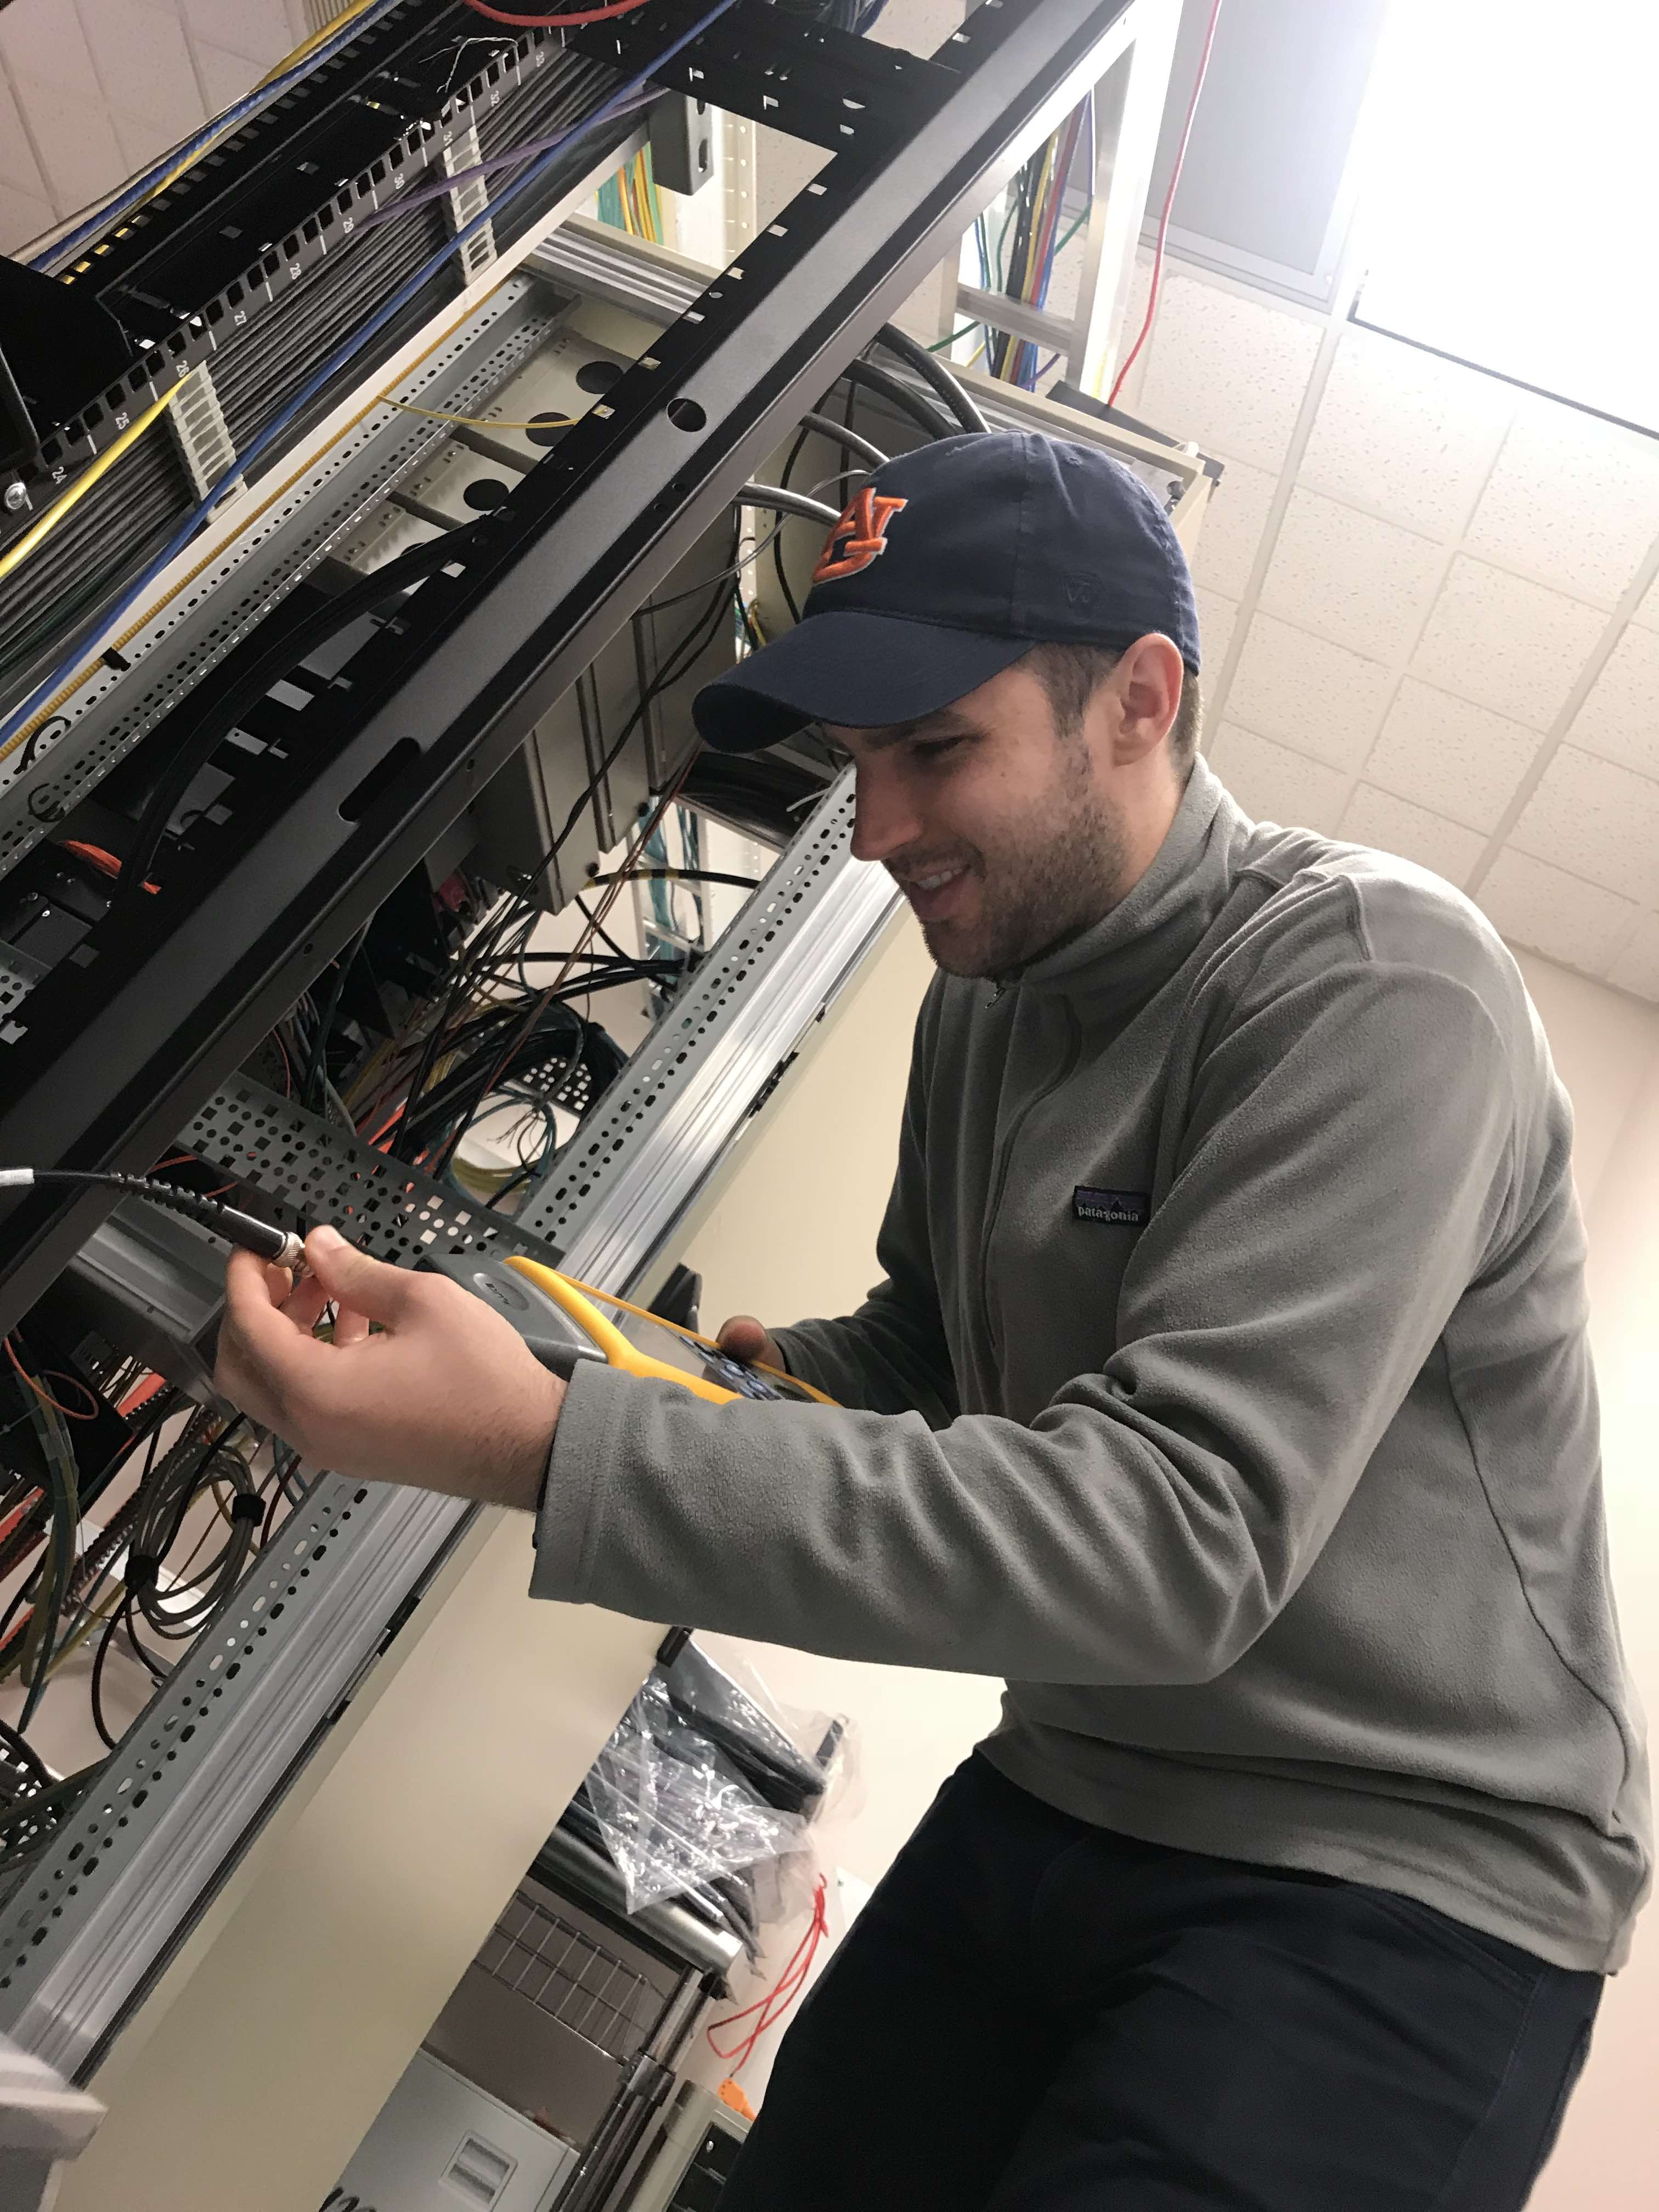
\includegraphics[width=0.8\linewidth]{img/rainer-performing-tdr.jpg}
	\end{center}
	\caption{Rainer Corley performing a Time Domain Reflectometry (TDR) cable length measurement on the cable running from the Symmetricom auxiliary GPS clock to the Timing Comparator (Aug. 2018).}
	\label{fig:rainertdr}
\end{figure}
\begin{figure}[!htb]
	\begin{center}
		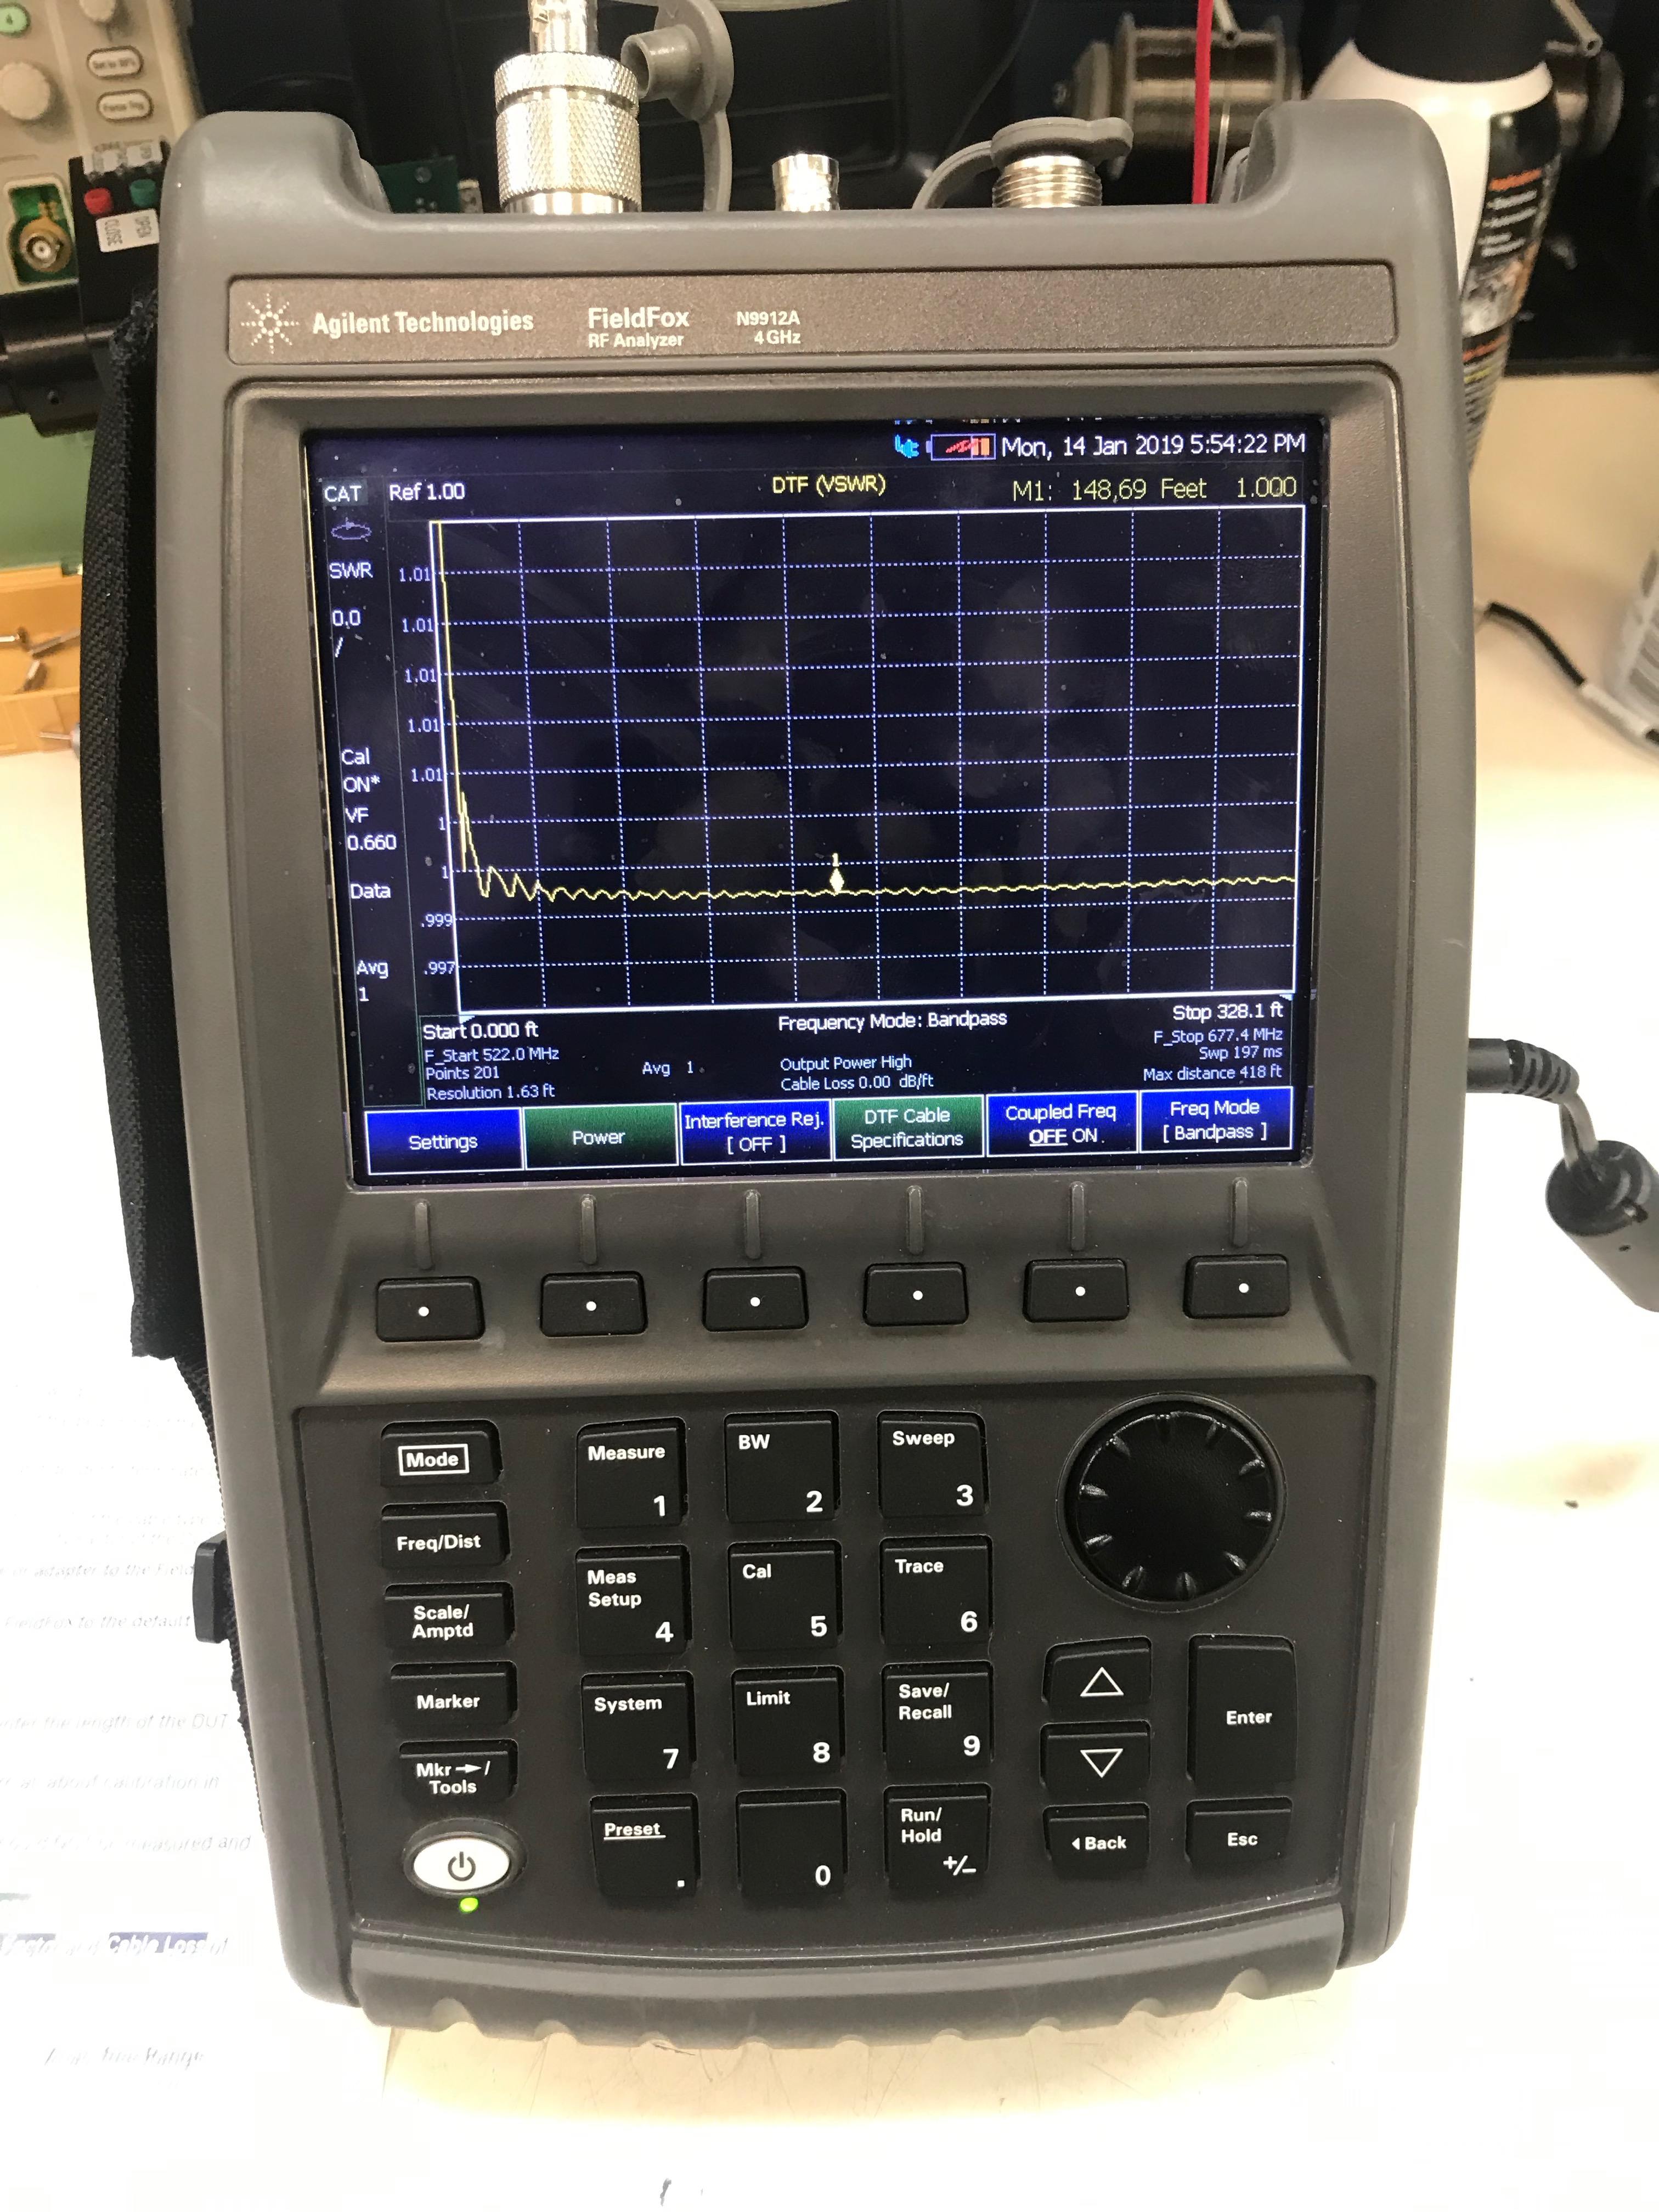
\includegraphics[width=0.8\linewidth]{img/time-domain-reflectrometer.jpg}
	\end{center}
	\caption{Device for performing \href{https://en.wikipedia.org/wiki/Time-domain_reflectometer}{Time Domain Reflectrometry} at LHO.}
	\label{fig:tdr-tool}
\end{figure}
\begin{figure}[!htb]
	\begin{center}
		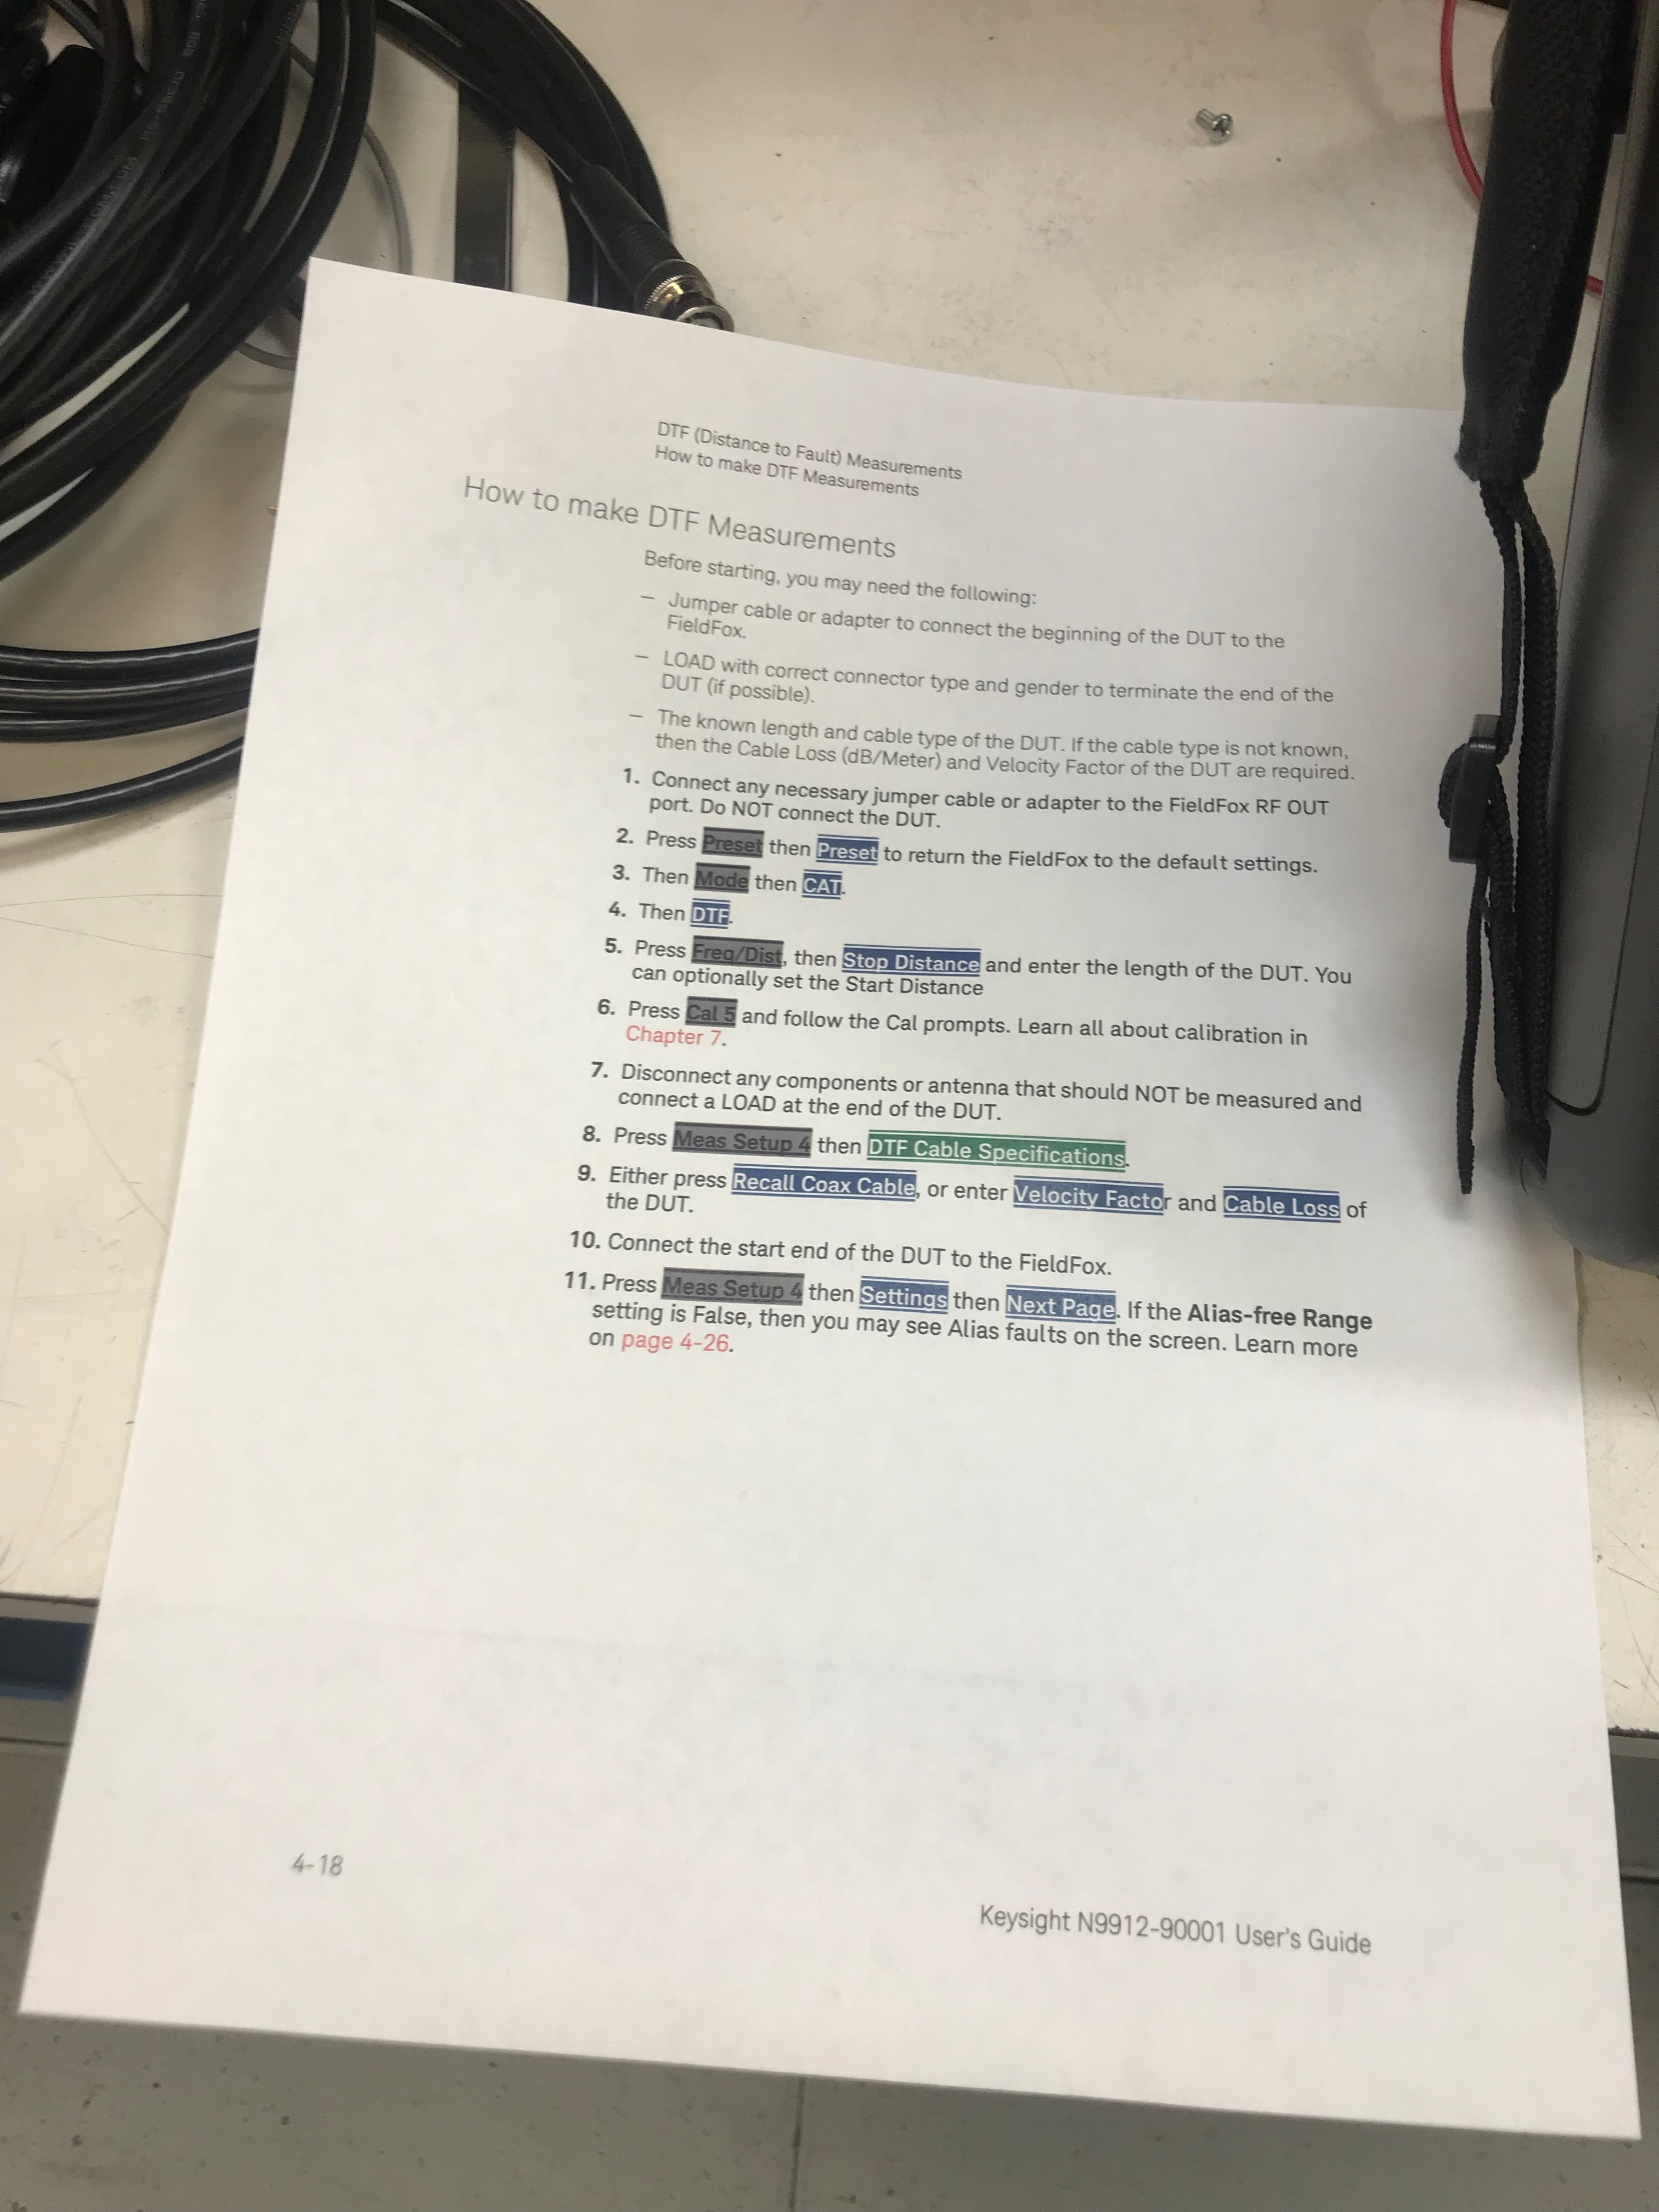
\includegraphics[width=0.8\linewidth]{img/time-domain-reflectrometer-dtf-instructions.jpg}
	\end{center}
	\caption{Instruction sheet for performing a DTF (Distance to Fault) distance measurement using this Time Domain Reflectrometer at LHO.}
	\label{fig:tdr-dtf-instructions}
\end{figure}
\begin{figure}[!htb]
	\begin{center}
		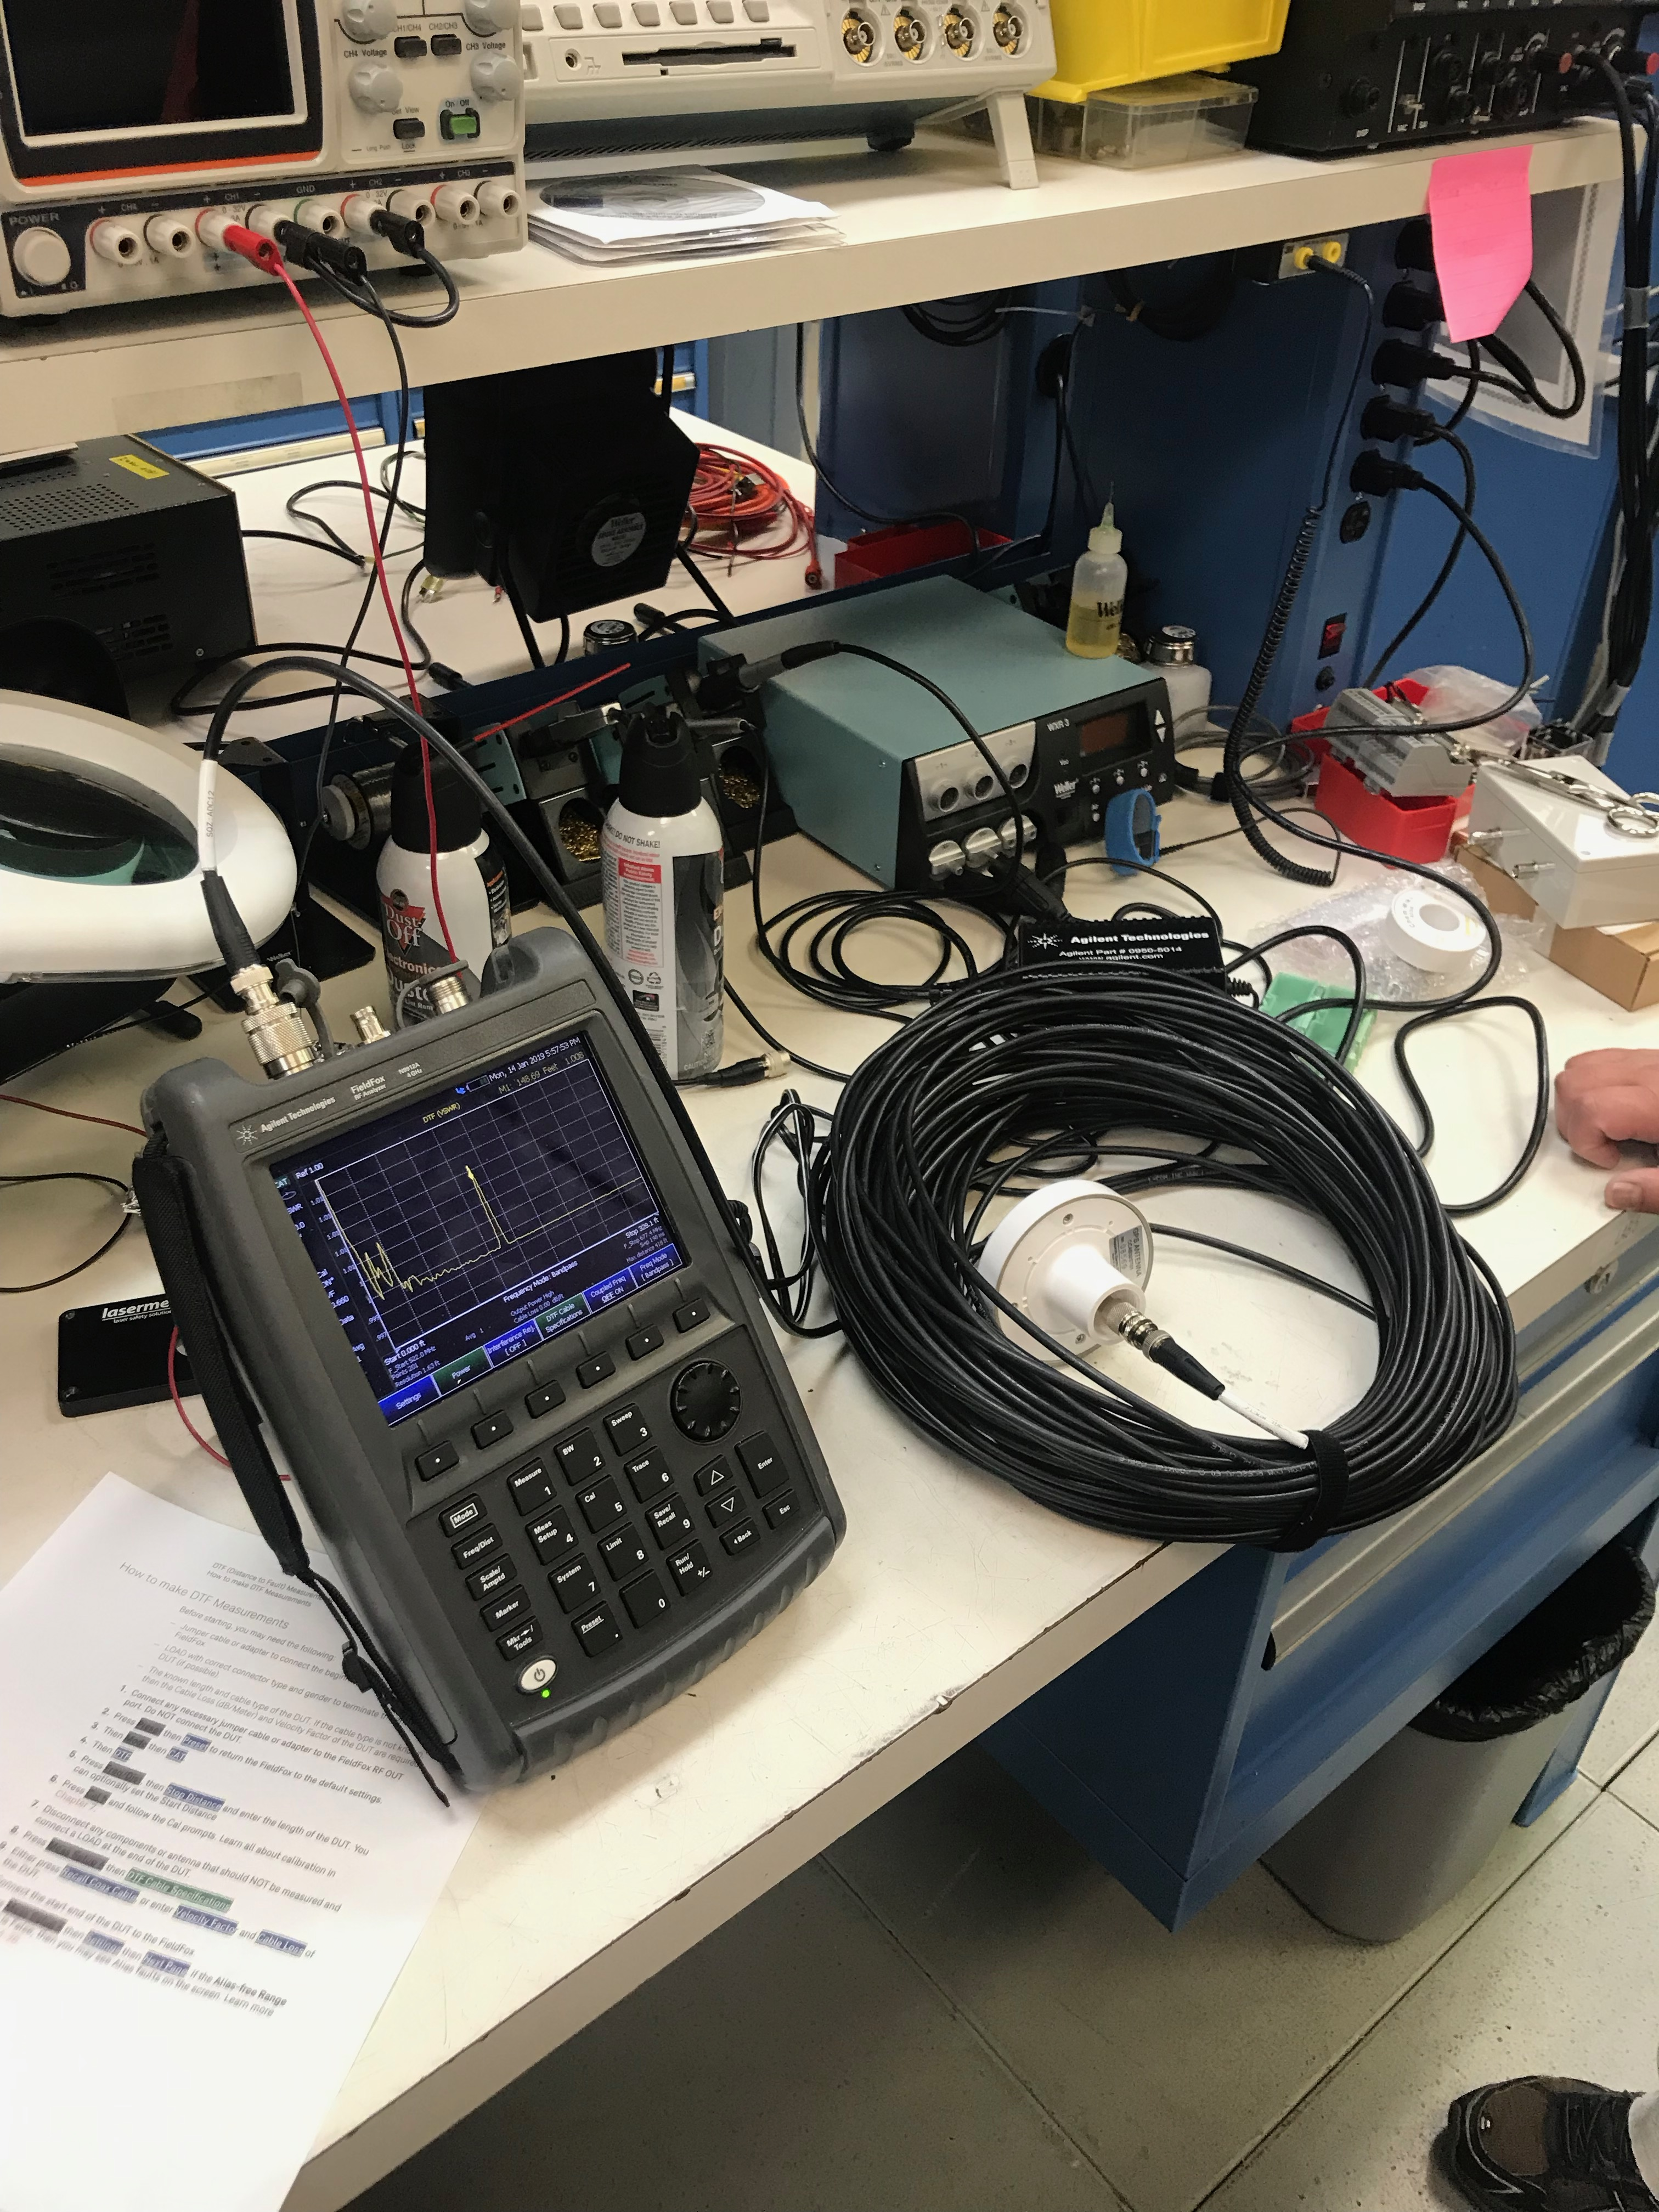
\includegraphics[width=0.8\linewidth]{img/time-domain-reflectrometer-dtf-test.jpg}
	\end{center}
	\caption{Proof of concept setup for measurement of a cable length terminated in a cable terminated by a GPS antenna.}
	\label{fig:tdr-test}
\end{figure}
\begin{figure}
	\begin{center}
		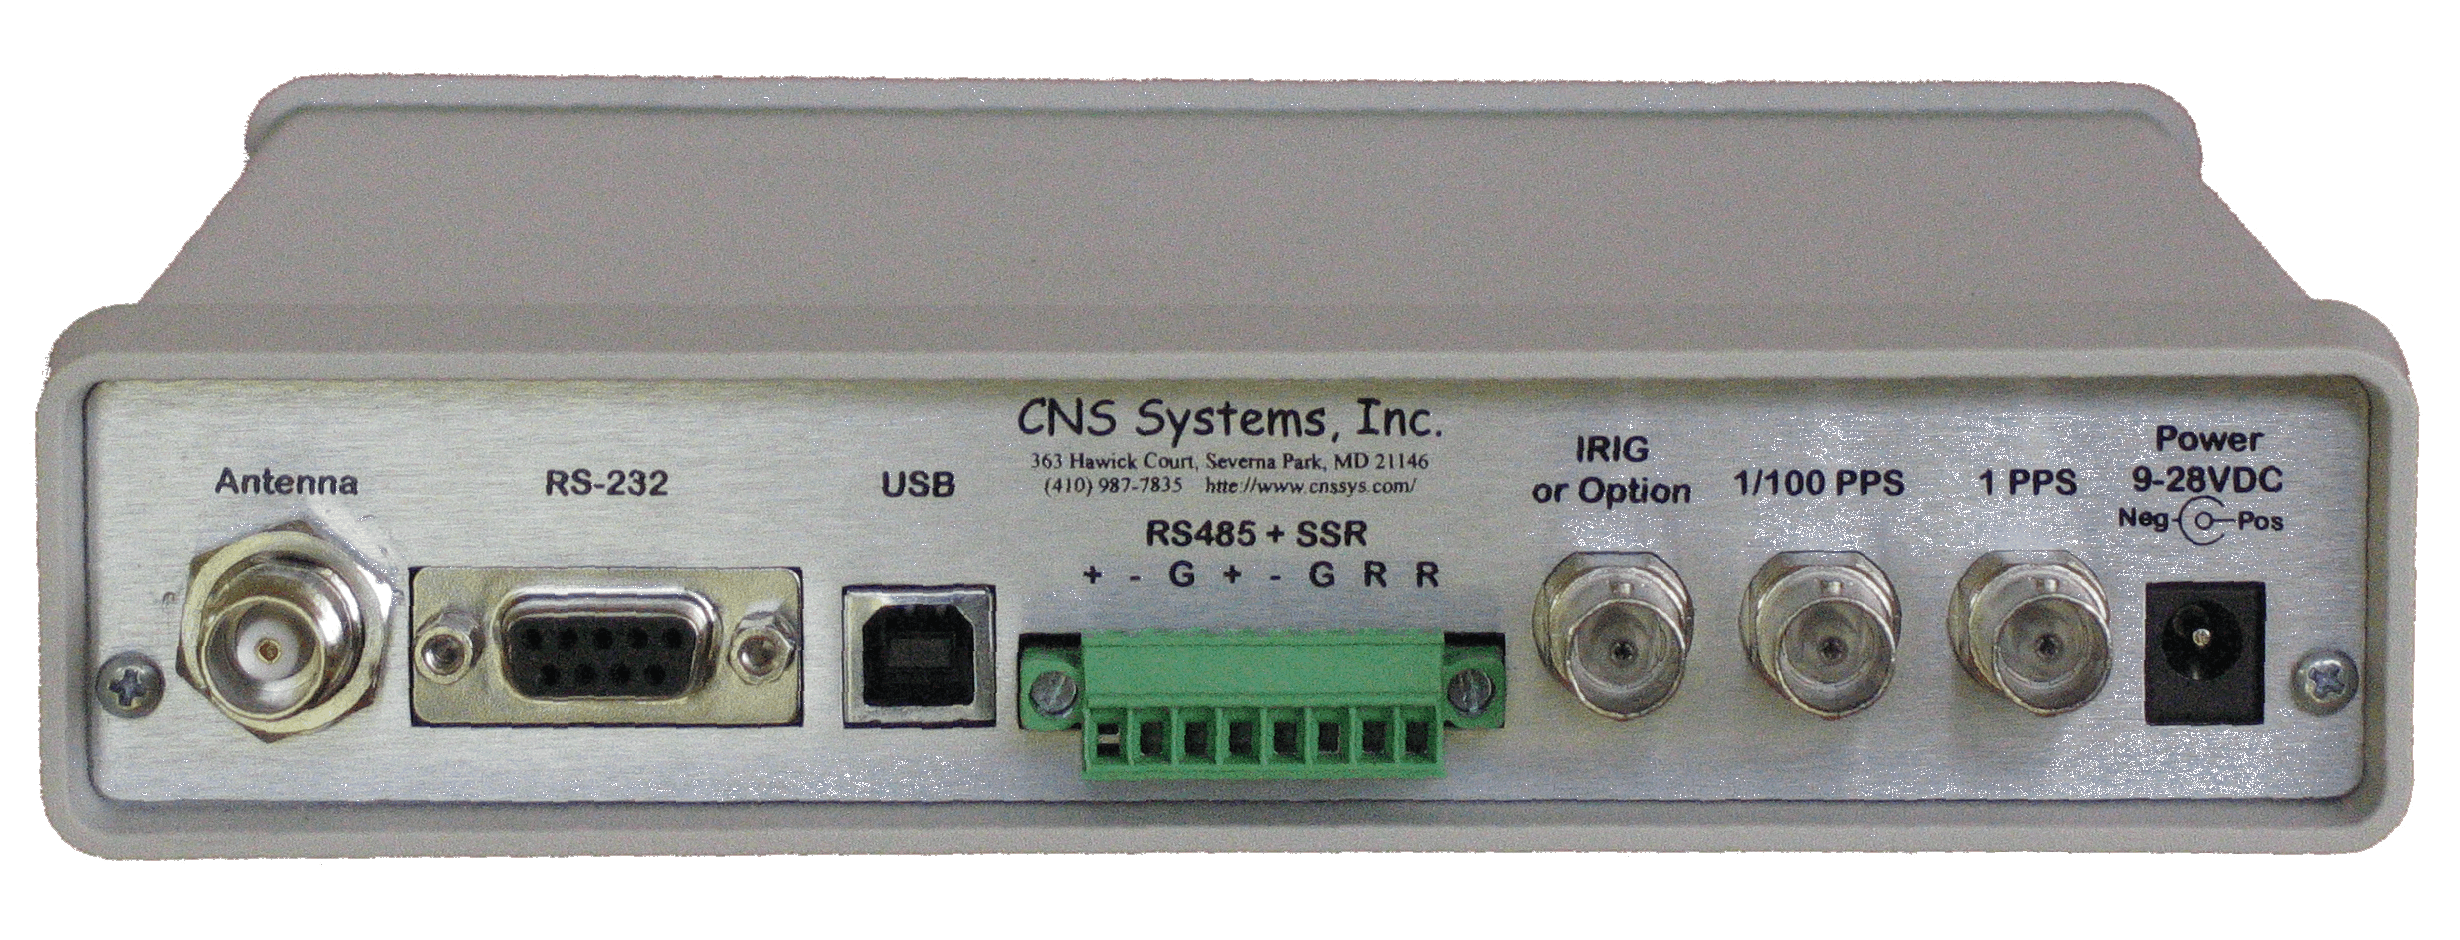
\includegraphics[width=0.8\linewidth]{img/cns-ii-rear.png}
	\end{center}
	\caption{The rear of the CNS II GPS clock which is installed at all end stations and is used for Diagnostic timing information.}
	\label{fig:cns-ii-rear}
\end{figure}
\begin{figure}
	\begin{center}
		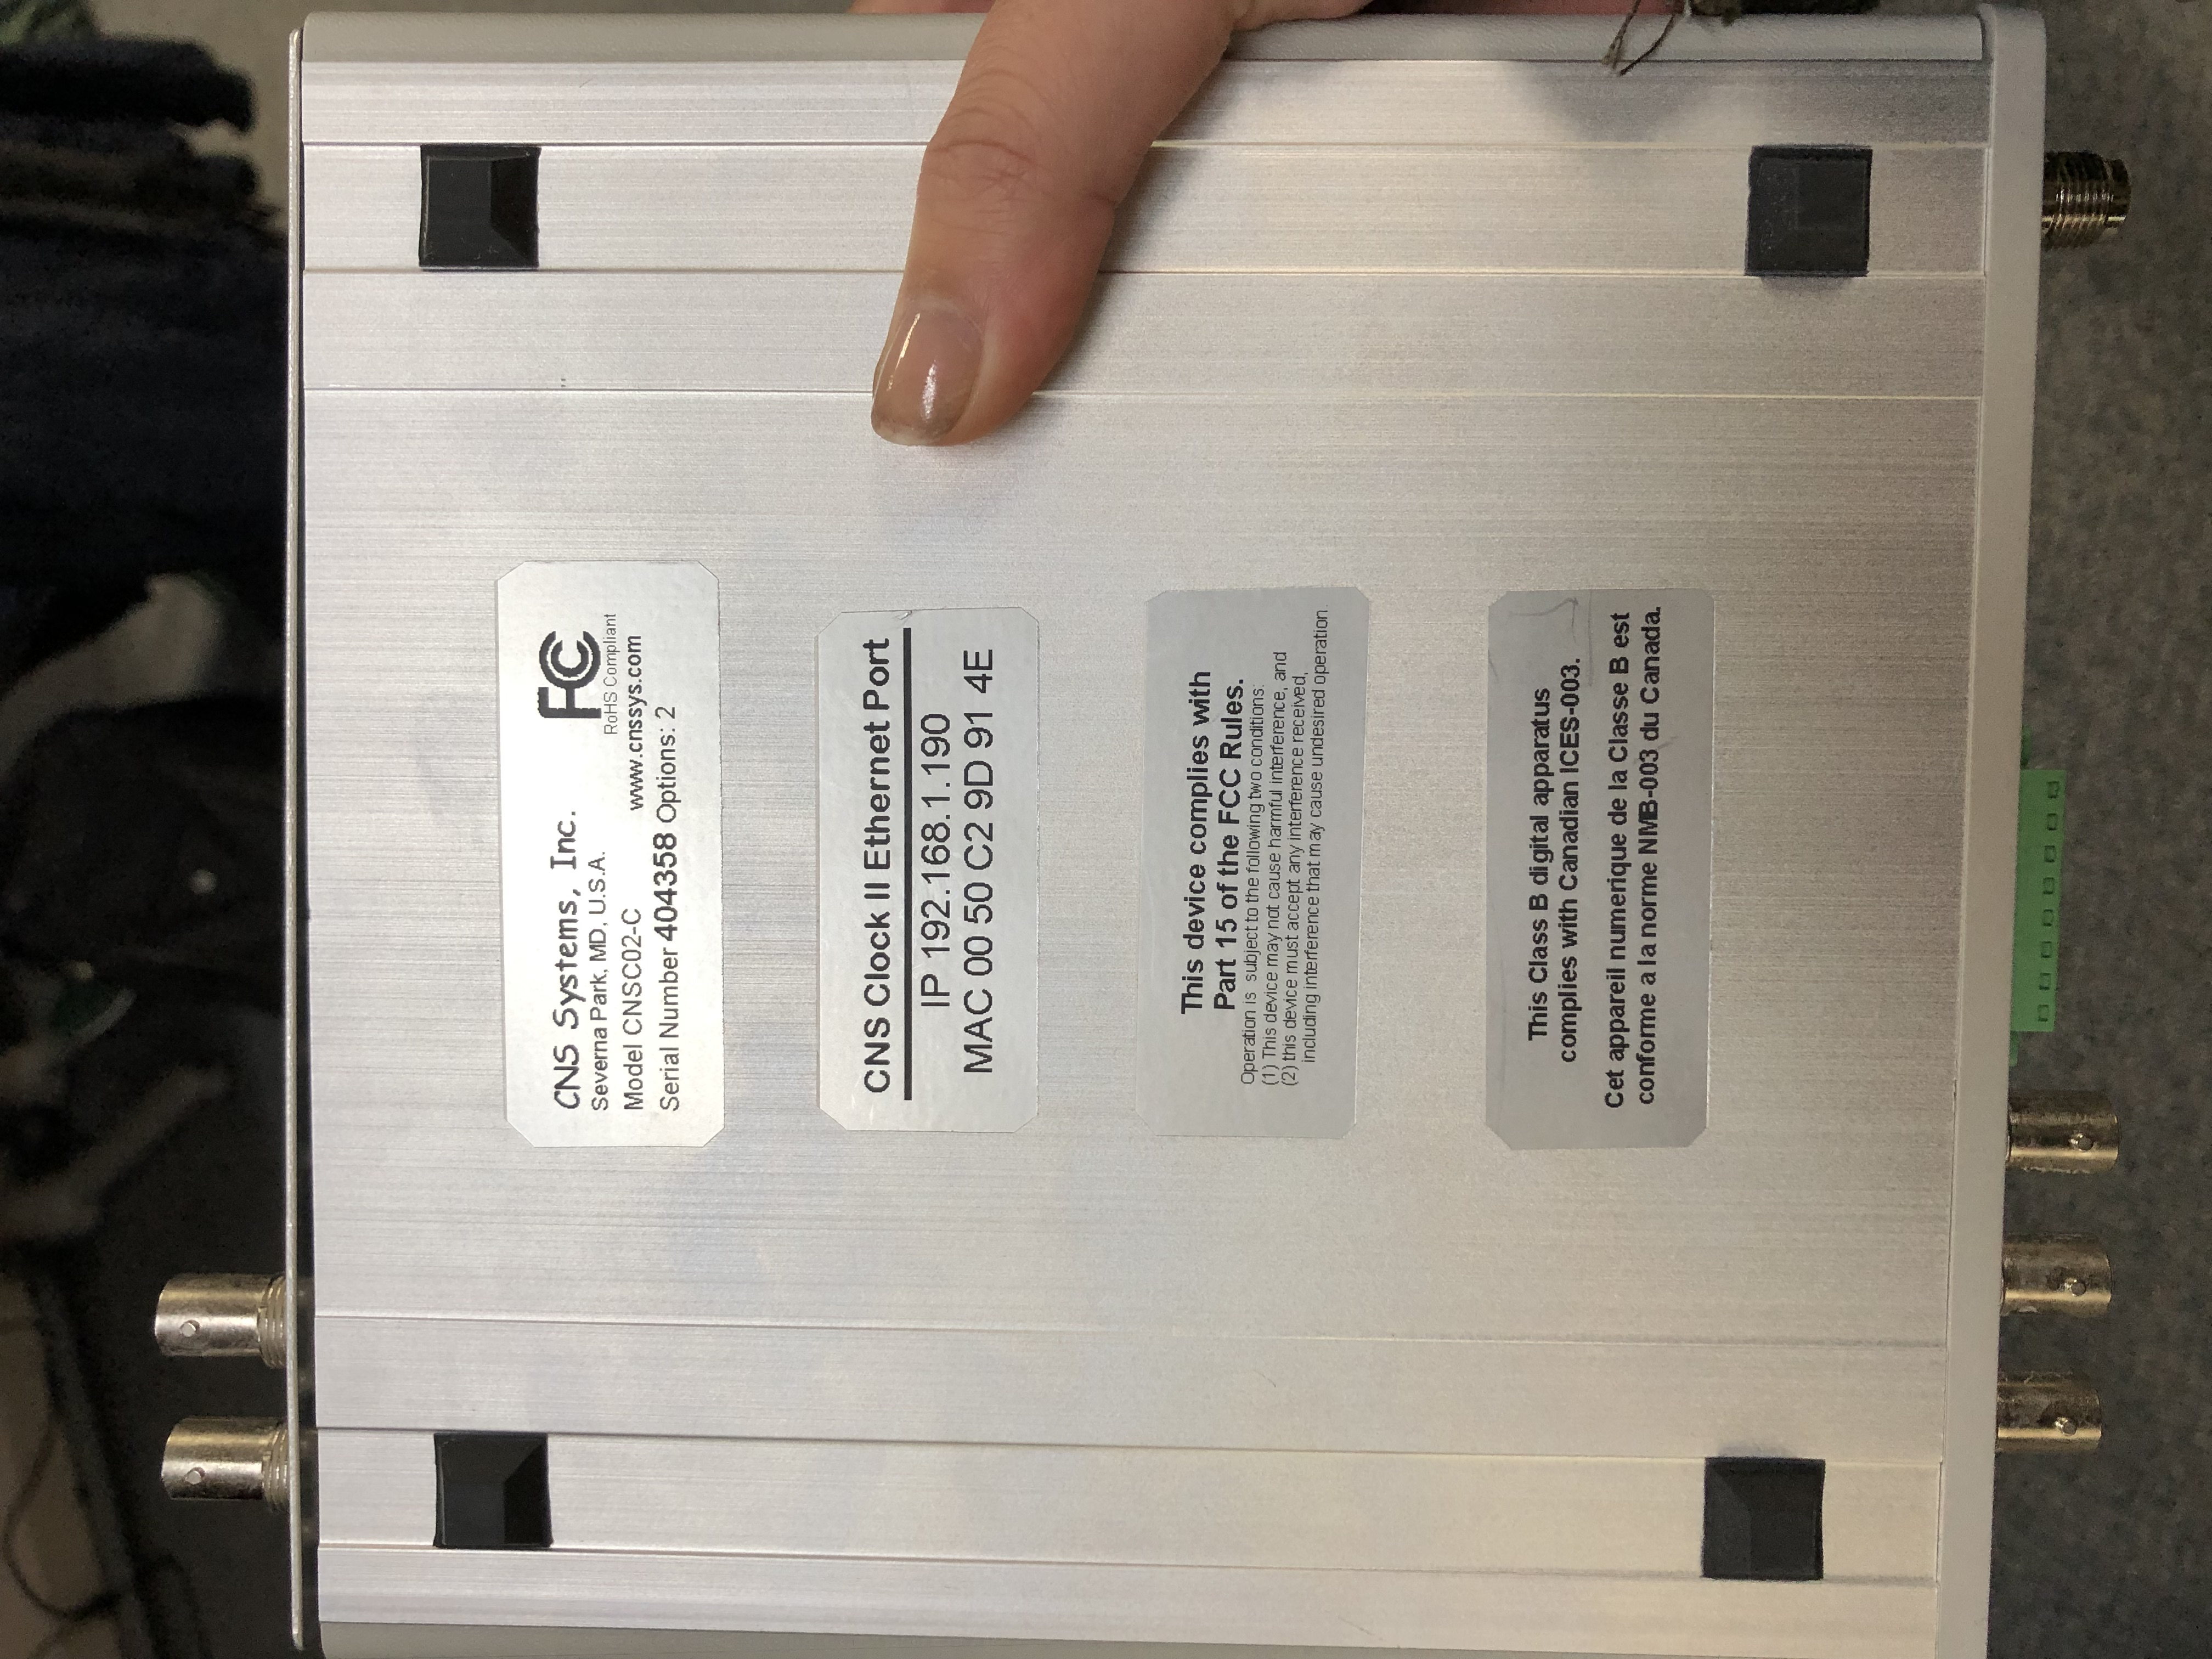
\includegraphics[width=0.8\linewidth]{img/cns-ii-ex-bottom-view.jpeg}
	\end{center}
	\caption{The Bottom of the X-End CNS-II Clock (removed for a firmware upgrade) displaying the serial number.}
	\label{fig:cns-ii-ex-bottom}
\end{figure}
\begin{figure}
	\begin{center}
		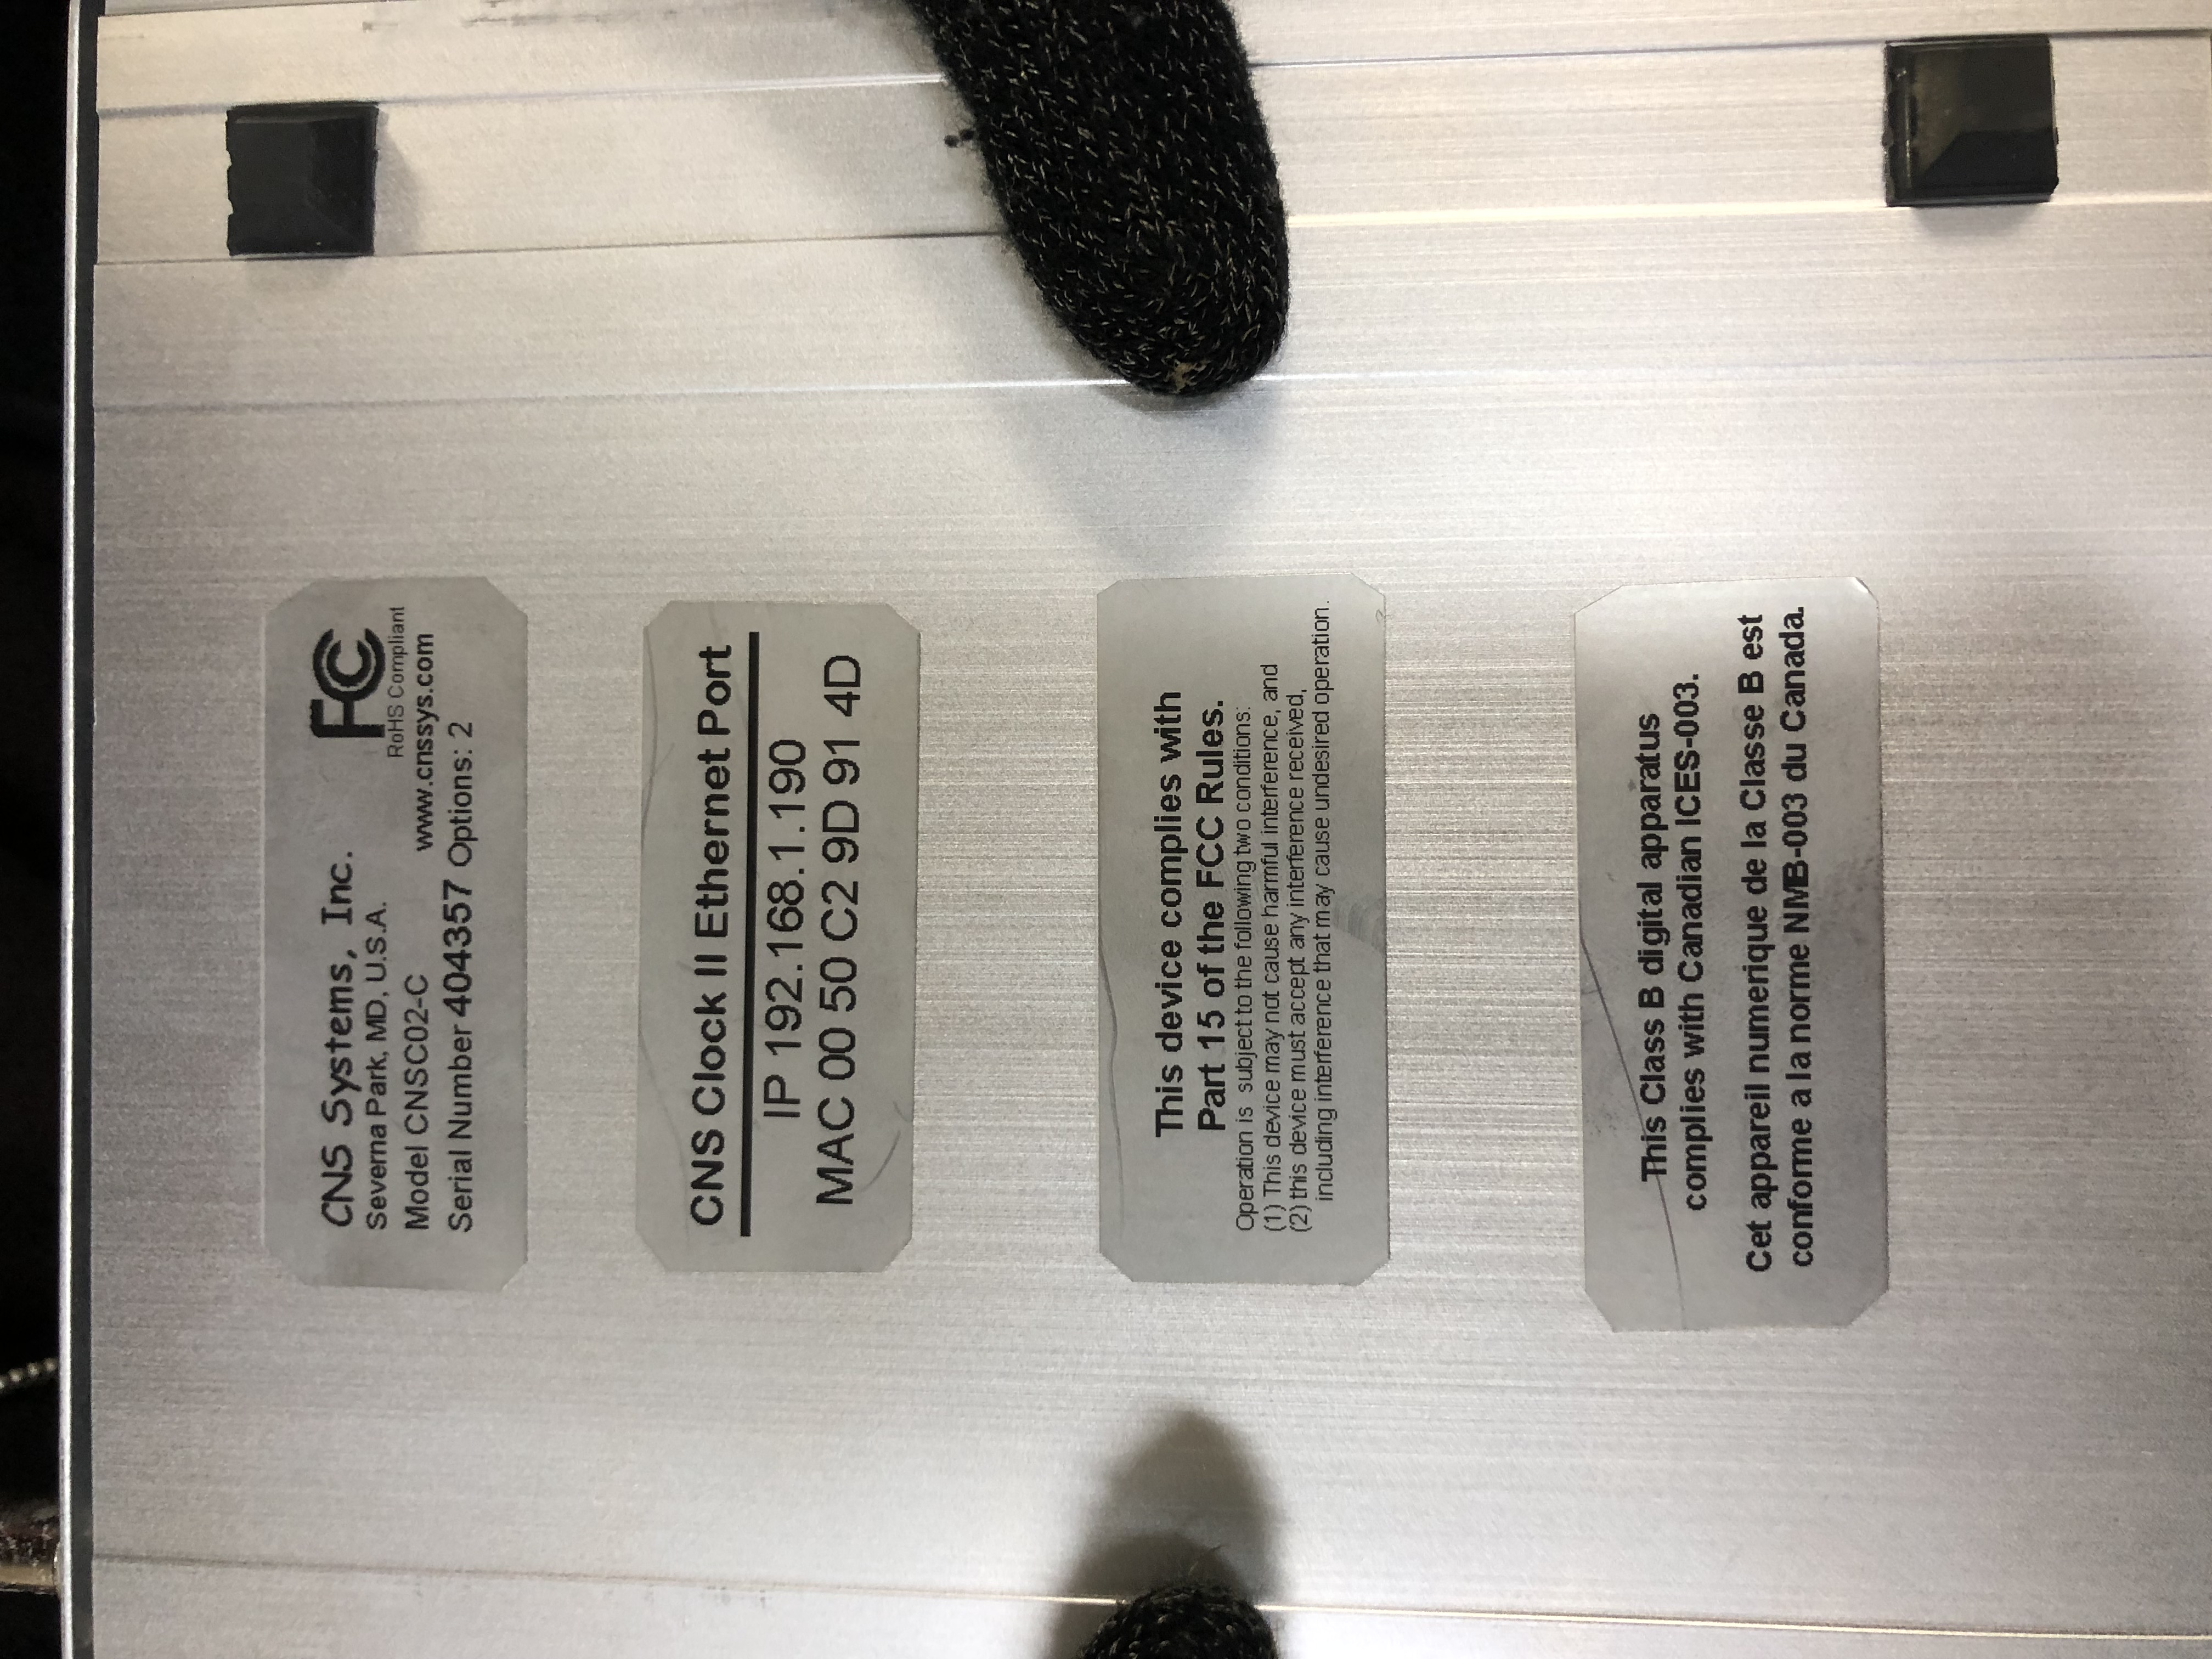
\includegraphics[width=0.8\linewidth]{img/cns-ii-ey-bottom-view.jpeg}
	\end{center}
	\caption{The Bottom of the Y-End CNS-II Clock (removed for a firmware upgrade) displaying the serial number.}
	\label{fig:cns-ii-ey-bottom}
\end{figure}
\begin{figure}
	\begin{center}
		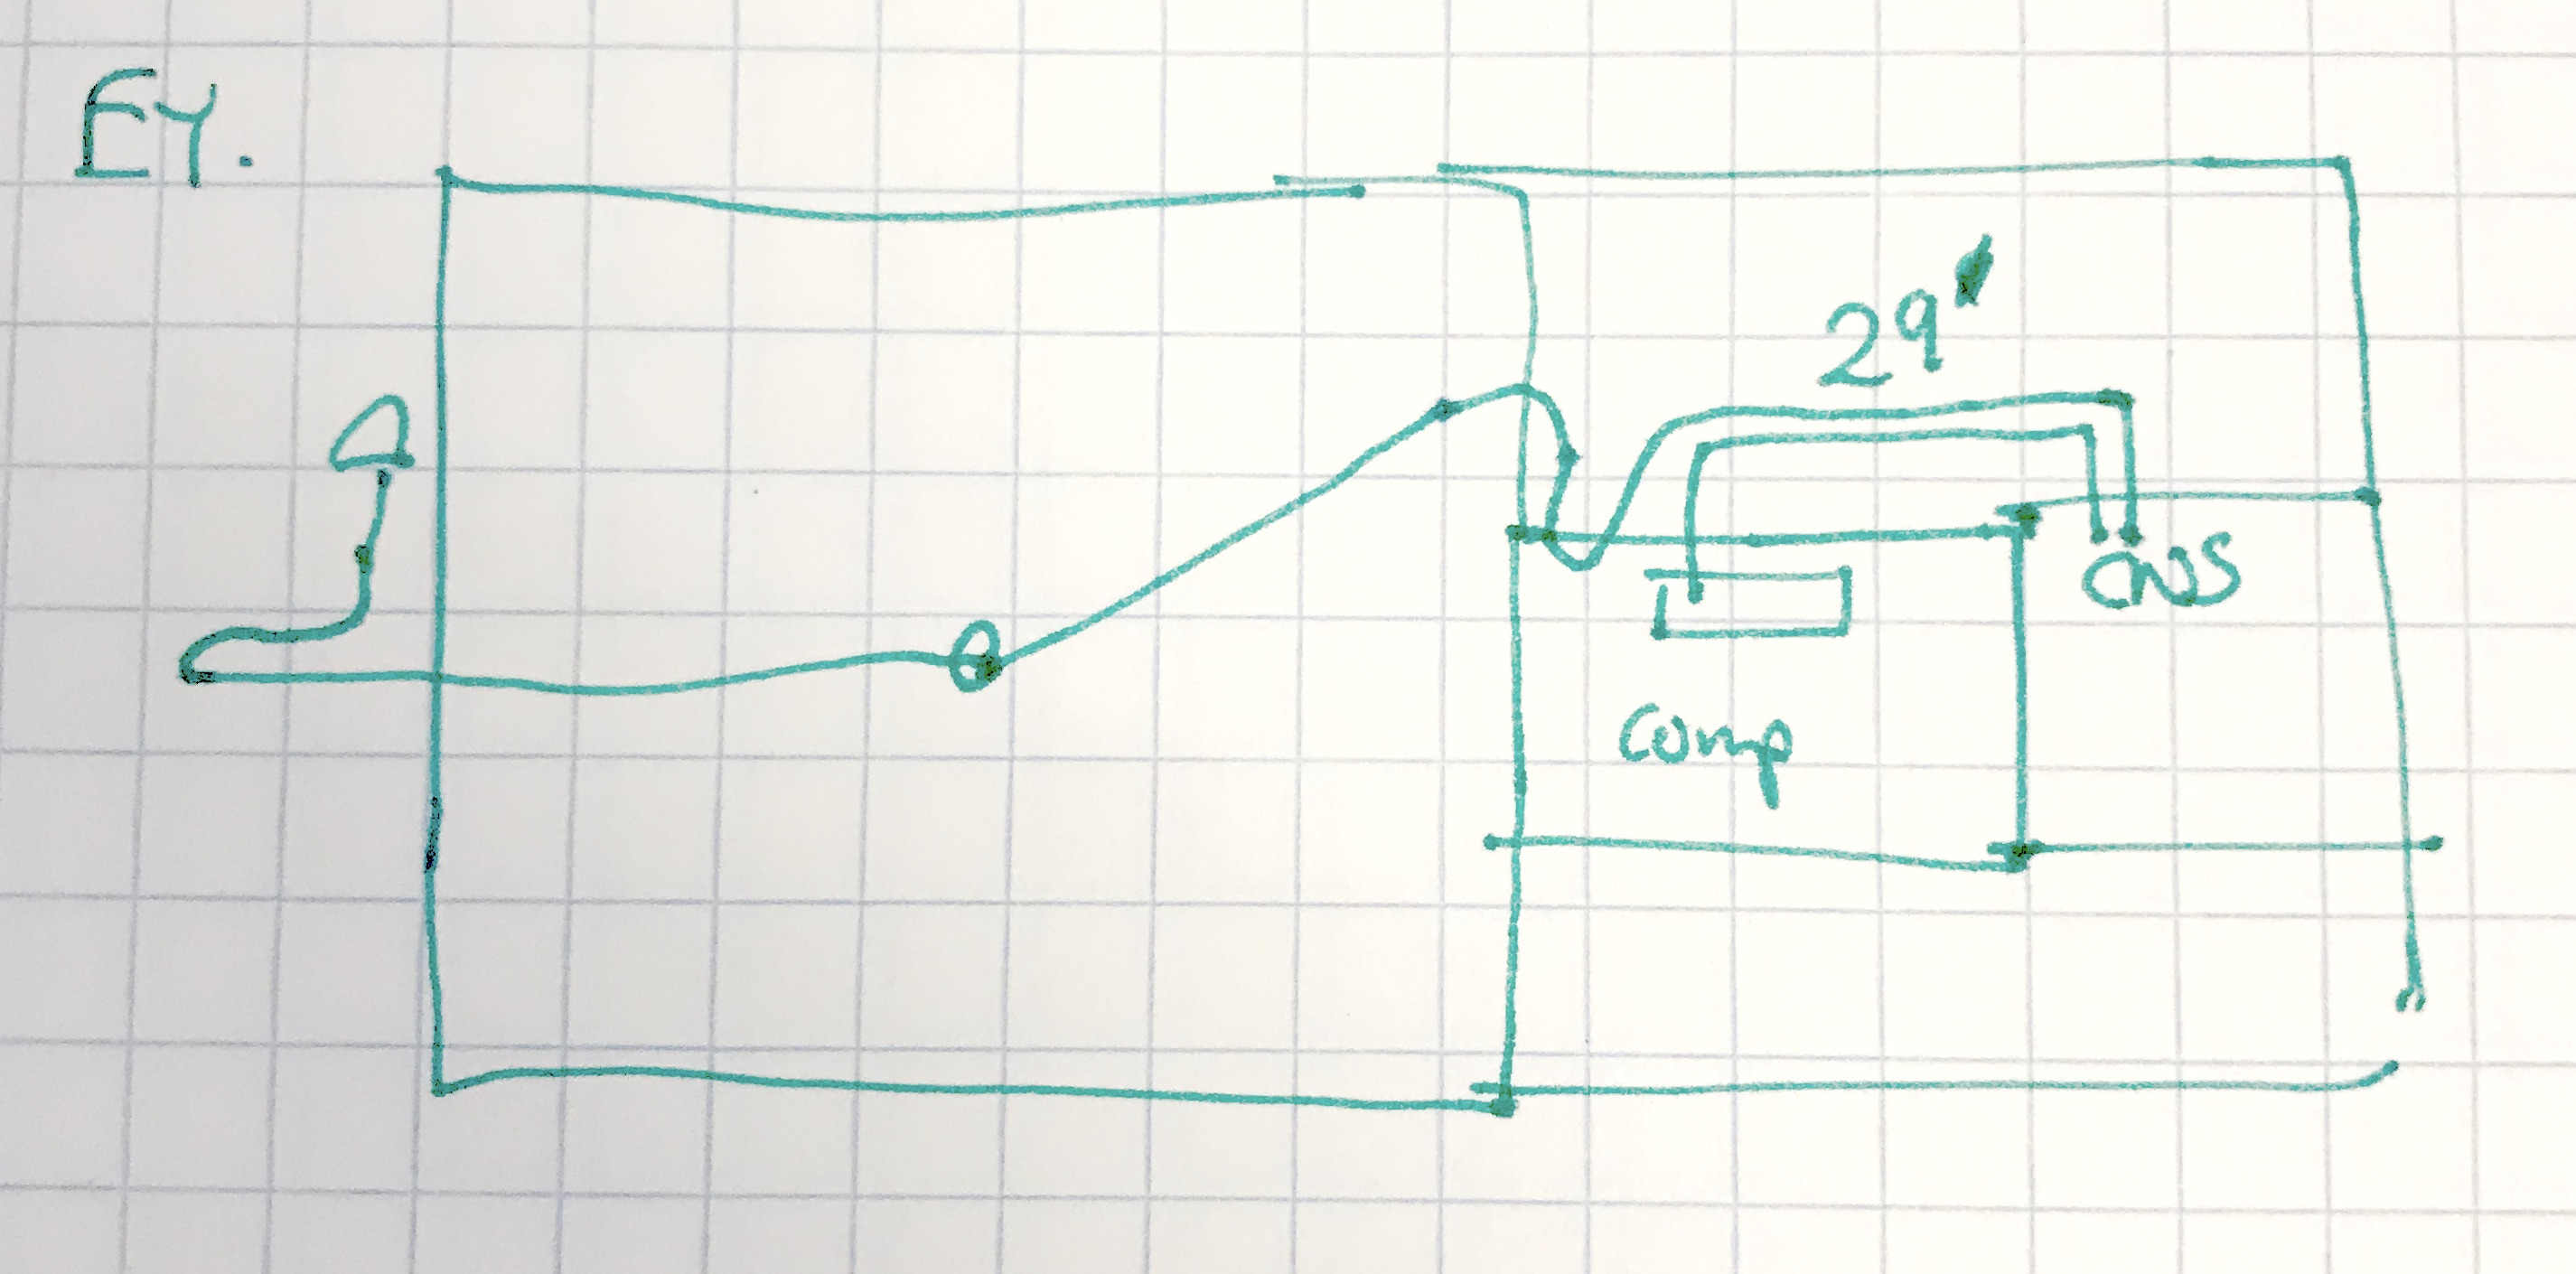
\includegraphics[width=0.8\linewidth]{img/endstation-antenna-cable.jpeg}
	\end{center}
	\caption{Cartoon by Dave Barker of CNS II GPS cable routing from clock to antenna in end stations. We can ask Dave for a more precise diagram/description if we really care about thse lengths.}
	\label{fig:routing}
\end{figure}
\begin{figure}
  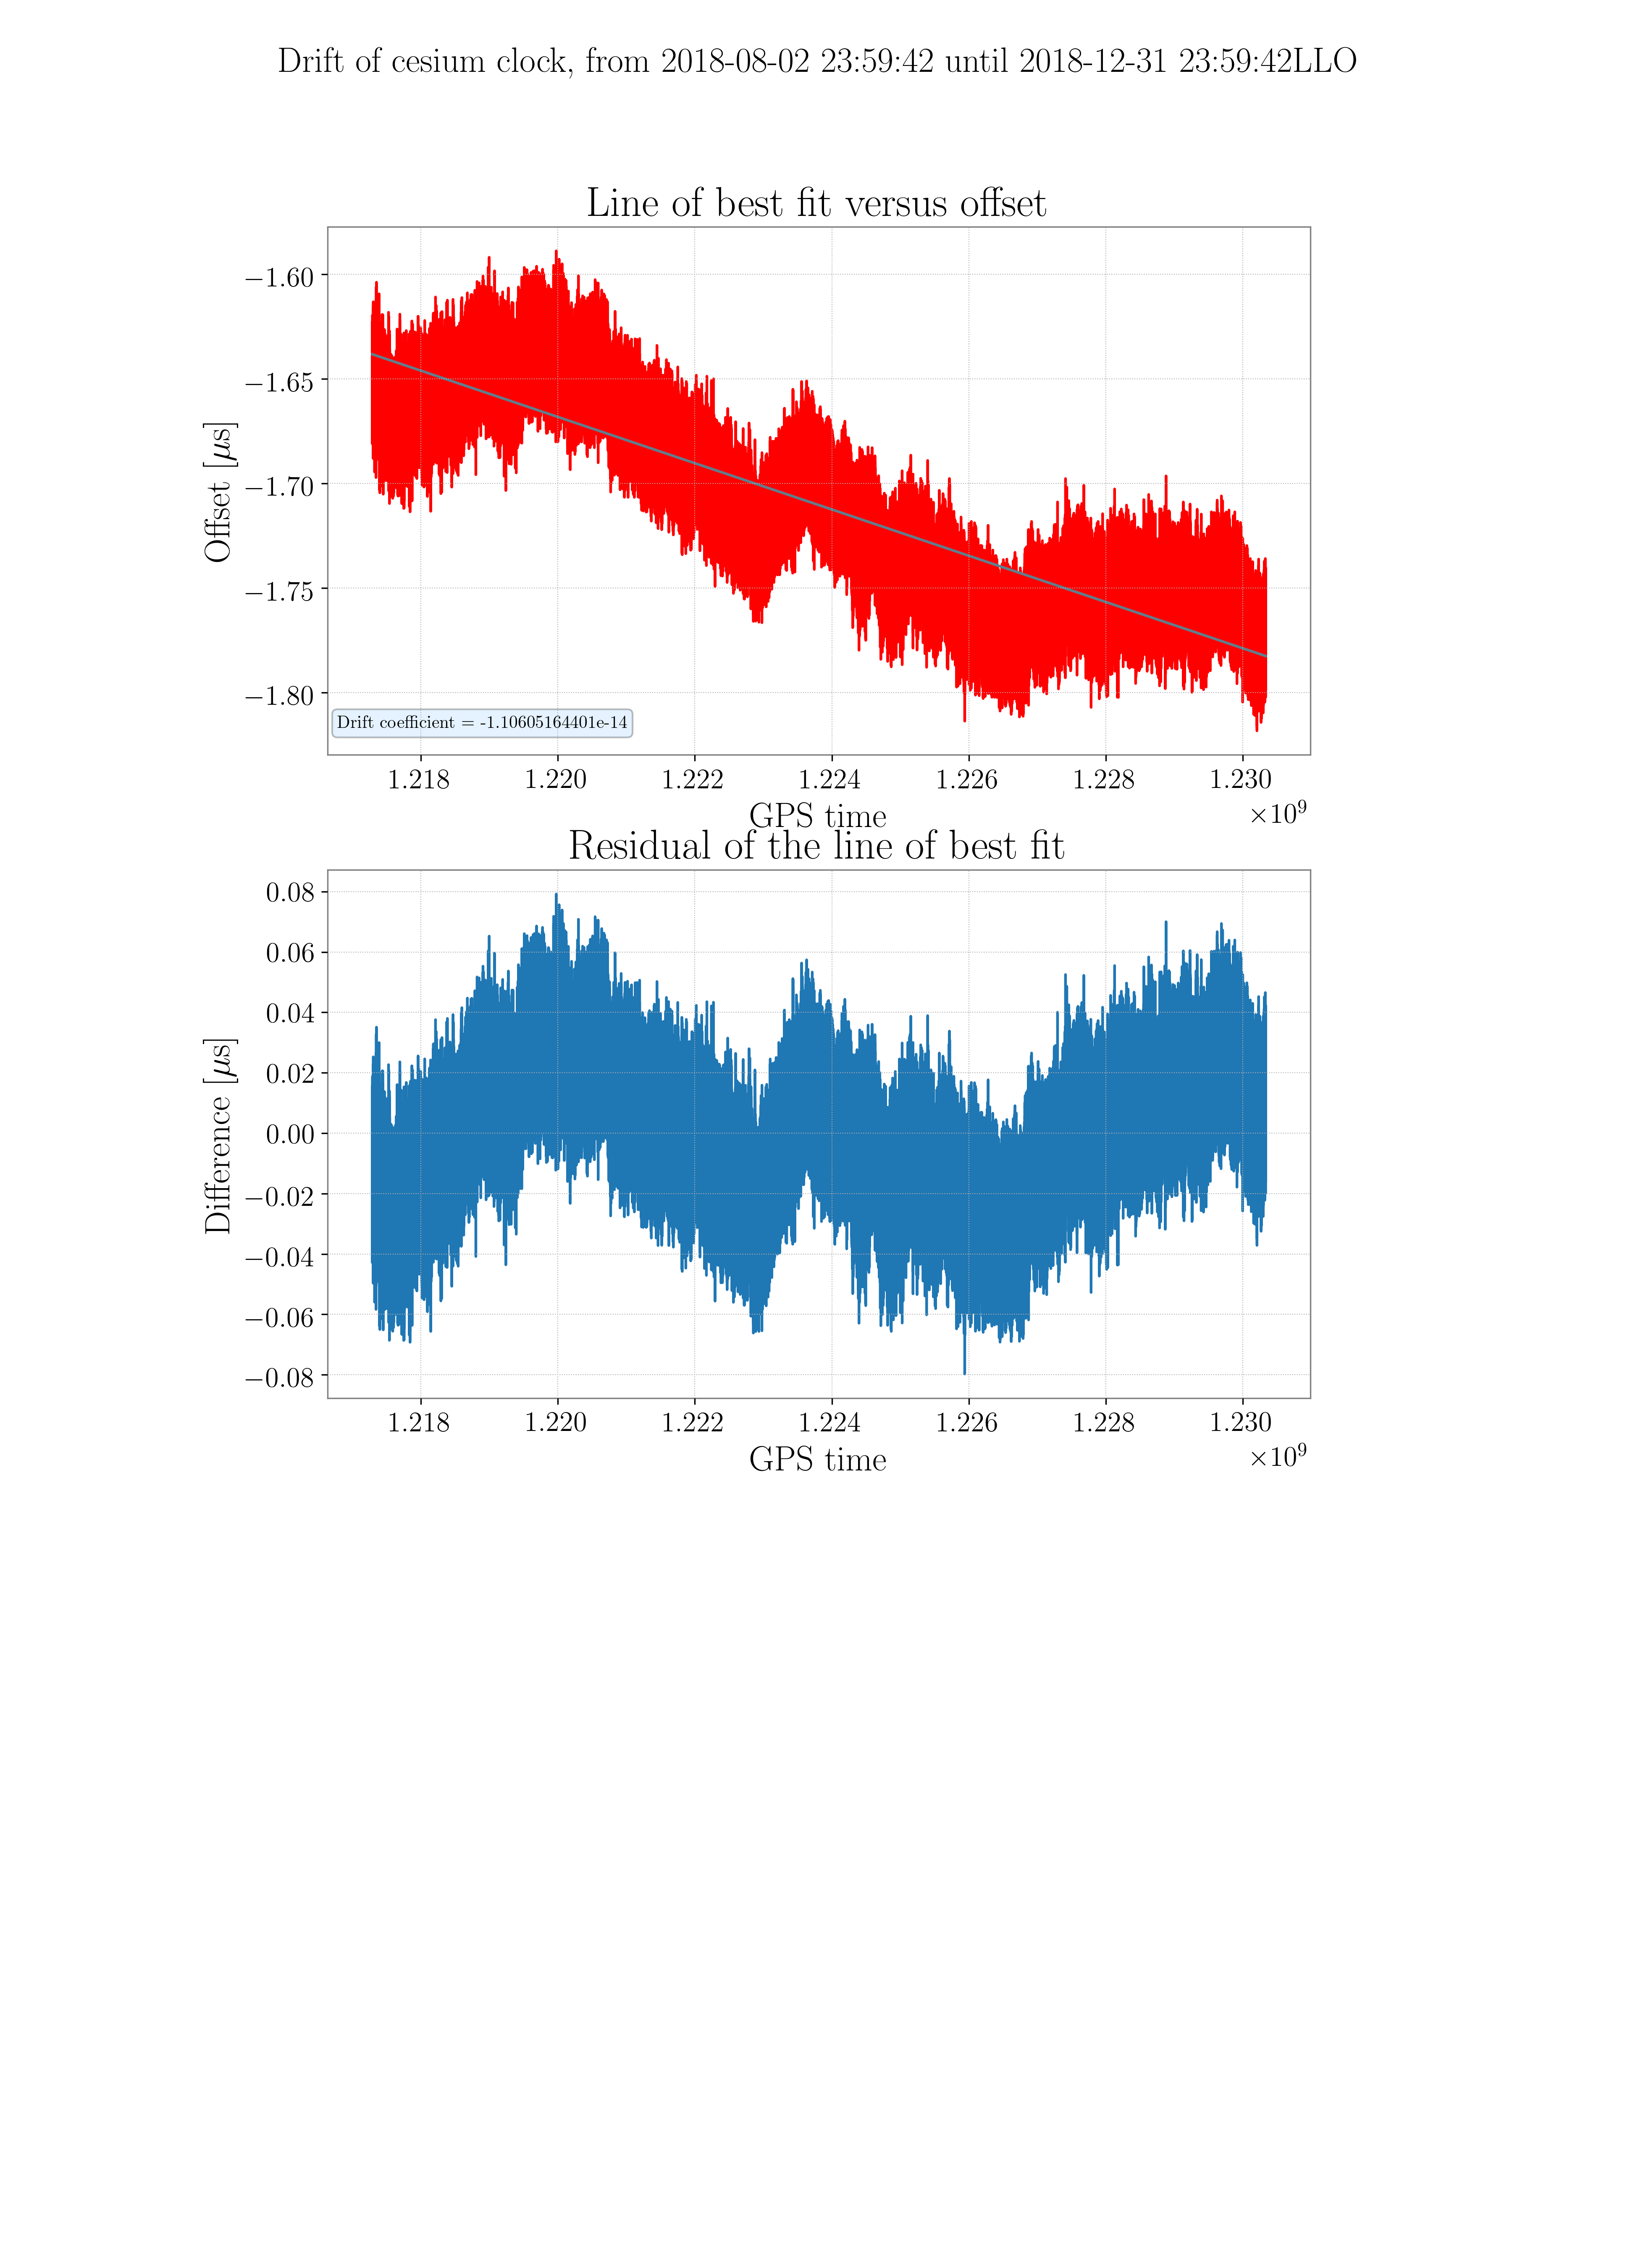
\includegraphics[width=\linewidth]{img/cesium-clock.png}
  \caption{Cesium 1PPS clock time difference vs. Timing System over last few months.}
  \label{fig:cesium}
\end{figure}
\begin{figure}
  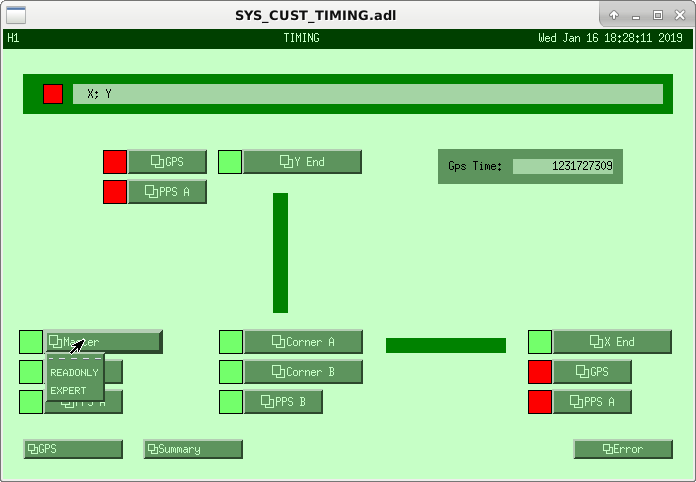
\includegraphics[width=\linewidth]{img/2019-01-16_lho-timing-overview-medm.png}
  \caption{Screenshot of the MEDM screens on-site showing the READONLY vs. EXPERT modes.}
  \label{fig:medm-expert-vs-readonly}
\end{figure}
\begin{figure}
  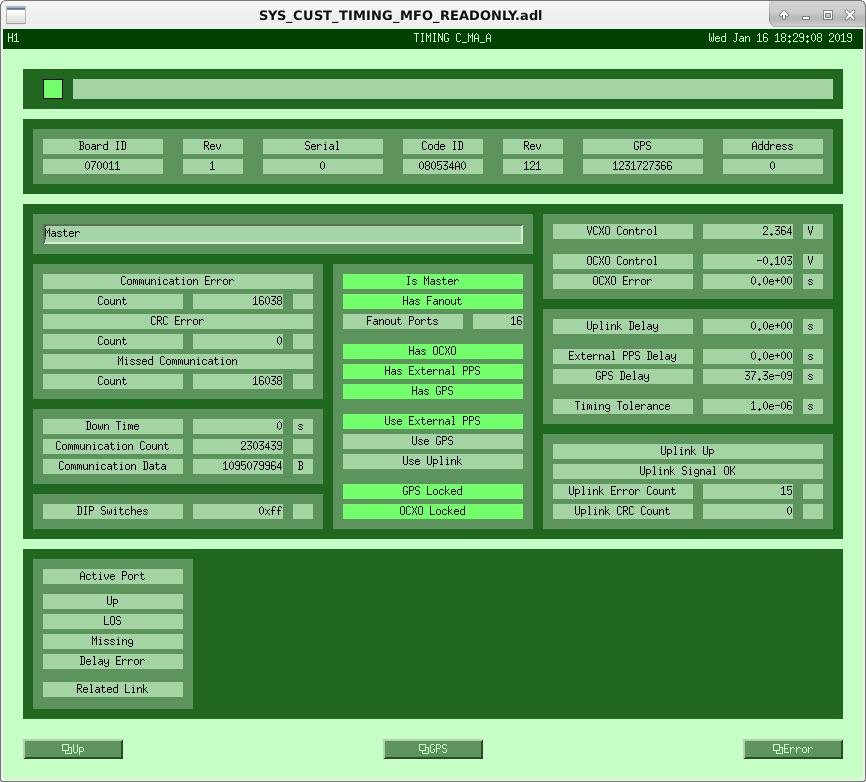
\includegraphics[width=\linewidth]{img/2019-01-16_lho-timing-master-readonly.png}
  \caption{Screenshot of the READONLY master MEDM screen (with the missing port information at the bottom).}
  \label{fig:medm-readonly}
\end{figure}
\begin{figure}
  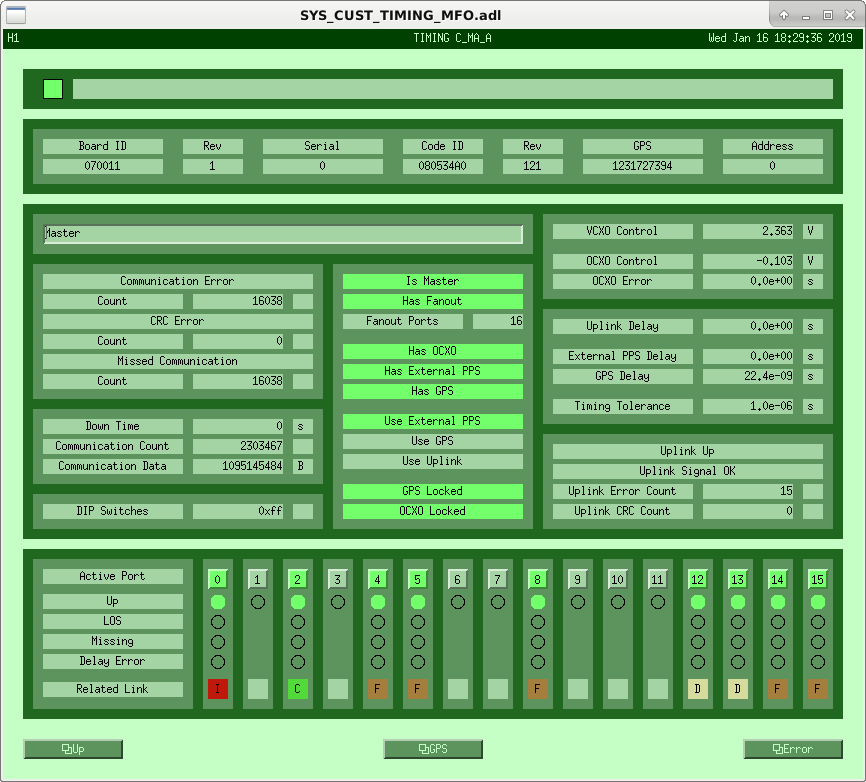
\includegraphics[width=\linewidth]{img/2019-01-16_lho-timing-master-expert.png}
  \caption{Screenshot of the EXPERT master MEDM screen (showing nominal behavior, i.e. port information at the bottom).}
  \label{fig:medm-expert}
\end{figure}
\clearpage

\section{LLO Cable Lengths}
\label{sec:llocables}
\begin{center}
  \begin{tabular}{ | l | l | l | l | }
    \hline
    \textbf{Cable Name}                 & \textbf{Type} & \textbf{Length (ft)}  & \textbf{Description} \\ \hline
    L1:TIM-EY\_GPS\_1PPS                & RG-58         & 18                    & Y-End CNS II 1PPS \\ \hline
    L1:TIM-EX\_GPS\_1PPS                & RG-58         & 20                    & X-End CNS II 1PPS \\ \hline
    L1:TIM-CSIII\_1PPS                  & RG-58         & 4                     & Cs-III 1PPS to rack plate \\ \hline
    1PPS GPS NTS                        & RG-58         & 3                     & NTP Server 1PPS to rack plate \\ \hline
    (No name)                           & RG-58         & 2                     & Rack plate Cs-III 1PPS to Comp. \\ \hline
    CAB\_L1:ACT-TTPPS\_012 (Repurposed) & RG-58         & 2                     & Rack plate NTP 1PPS to Comparator \\ \hline
                                        & LMR-400       & 0                     & Timing Master GPS Antenna Cable \\ \hline
    TRIMBLE ANTENNA                     & LMR-400       & 0                     & Trimble GPS Antenna Cable \\ \hline
    GPS ANT                             & LMR-195       & 0                     & Y-End CNS II GPS Antenna Cable \\ \hline
    GPS ANT                             & LMR-195       & 0                     & X-End CNS II GPS Antenna Cable \\ \hline
    H1:DAQ (Repurposed)                 & RG-58         & 1                     & Trimble to Master 1PPS cable \\ \hline
    (No name)                           & RG-58         & 2                     & 58539A Lightning arrestor to Trimble \\ \hline
    (No name)                           & RG-58         & 3                     & 58539A Lightning arrestor to Master \\ \hline
  \end{tabular}
\end{center}
\clearpage

\section{Firmware Version Information for Timming FPGAs}
\label{sec:firmware}
\begin{center}
  \begin{tabular}{ | l | l | l | l | }
    \hline
    \textbf{MFO Module}                 & \textbf{Number of FPGAs} & \textbf{SVN Revision}  & \textbf{Recommendation} \\ \hline
    Master                & 1         & 121                    & Production \\ \hline
    Master: Duotones                & 2         & 118                    & Production \\ \hline
    Master: IRIG-B                & 1         & 118                    & Production \\ \hline
    Master: Comparator                & 1         & 125                    & Production \\ \hline
    Master: FanOuts              & 5         & 121                    & Production \\ \hline
    Corner A                & 1         & 121                    & Production \\ \hline
    Corner A: Duotones                  & 7         & 118                     & Production \\ \hline
    Corner A: RF Ocsillators                        & 5         & 118                     &  Production\\ \hline
    Corner A: C                           & 1         & 125                     & Production \\ \hline
    Corner B   & 1         & 121                     & Production \\ \hline
    Corner B: Duotones                            & 13       & 118                     & Production \\ \hline
    Y-End                     & 1       & 121                     & Production \\ \hline
    Y-End: IRIG-B                             & 1       & 118                     & Production \\ \hline
    Y-End: Duotones                             & 4       & 118                     & Production \\ \hline
    Y-End: RF Oscillators                 & 2         & 118               & Production \\ \hline
    Y-End: C                           & 1         & 125                     & Production \\ \hline
    X-End                     & 1       & 121                     & Production \\ \hline
    X-End: IRIG-B                             & 1       & 118                     & Production \\ \hline
    X-End: Duotones                             & 4       & 118                     & Production \\ \hline
    X-End: RF Oscillators                 & 2         & 118            &  Production \\ \hline
    X-End: C                           & 1         & 125                     & Production \\ \hline
  \end{tabular}
\end{center}
\clearpage

\end{document}
